% VAMOS Paper: IEEE Transactions on Evolutionary Computation (IEEE TEVC)
% =============================================================================
% Supplementary Material
% =============================================================================
\documentclass[journal]{IEEEtran}

\usepackage{cite}
\usepackage{graphicx}
\usepackage{booktabs}
\usepackage{amsmath}
\usepackage{amssymb}
\usepackage{multirow}
\usepackage{algorithm}
\usepackage{algpseudocode}
\usepackage{listings}
\usepackage{xcolor}
\usepackage{pifont}
\usepackage{enumitem}
\usepackage{stfloats}
\newcommand{\cmark}{\ding{51}}
\newcommand{\pmark}{\ding{109}}
\newcommand{\xmark}{\ding{55}}
\usepackage[hidelinks]{hyperref}
\hypersetup{hypertexnames=false}
\makeatletter
\g@addto@macro\UrlBreaks{\do\.\do\_\do\-\do\/}
\makeatother

% Code listing style
\lstset{
  language=Python,
  basicstyle=\ttfamily\footnotesize,
  keywordstyle=\color{blue},
  commentstyle=\color{gray},
  stringstyle=\color{red!70!black},
  showstringspaces=false,
  frame=single,
  breaklines=true,
  numbers=left,
  numberstyle=\tiny\color{gray}
}

\newcommand{\VAMOS}{VAMOS}
\newcommand{\HV}{\mathrm{HV}}
\newcommand{\Intdomain}[1]{[#1]_{\mathbb{Z}}}
\newcommand{\Realdomain}[1]{[#1]_{\mathbb{R}}}

\title{Supplementary Material: A High-Performance Vectorized Framework for Multiobjective Evolutionary Optimization in Python}

% --------------------------------------------------------------------------
%  Author block.
% --------------------------------------------------------------------------
\author{Nicol\'{a}s~R.~Uribe,
        Alberto~Herr\'{a}n,
        Antonio~J.~Nebro,
        Javier~Del~Ser,
        and~J.~Manuel~Colmenar%
\thanks{N. R. Uribe, A. Herr\'{a}n, and J. M. Colmenar are with the
  Department of Computer Sciences, Universidad Rey Juan Carlos, M\'{o}stoles,
  28933 Madrid, Spain (e-mail: nicolas.rodriguez@urjc.es; alberto.herran@urjc.es;
  josemanuel.colmenar@urjc.es).}%
\thanks{A. J. Nebro is with the Department of Lenguajes y Ciencias de la
  Computaci\'{o}n, ITIS Software, University of M\'{a}laga, 29071
  M\'{a}laga, Spain (e-mail: ajnebro@uma.es).}%
\thanks{J. Del Ser is with TECNALIA, Basque Research \& Technology
  Alliance (BRTA), Derio, 48160, Spain, and also with the University
  of the Basque Country (UPV/EHU), Leioa, 48940, Spain (e-mail: javier.delser@tecnalia.com).}%
\thanks{Corresponding author: Alberto Herr\'{a}n (alberto.herran@urjc.es).}%
}

\markboth{IEEE Transactions on Evolutionary Computation}%
{A Vectorized Framework for Multiobjective Evolutionary Optimization}

\begin{document}
\maketitle

%==============================================================================
\appendices
\section{Additional runtime comparisons}
\label{app:variants}
Tables in this appendix report supplementary runtime comparisons for NSGA-II variants (steady-state and external archive), SMS-EMOA, and MOEA/D under the same protocol as the Experimental Results section of the main paper.

% Auto-generated by paper/14_update_frameworks_perf_variant_tables_from_csv.py

\begin{table}[htbp]
\centering
\caption{Median runtime (seconds) by problem family for algorithm variants}
\label{tab:frameworks_perf_variants}
\begin{tabular}{llcccc}
\toprule
\textbf{Algorithm} & \textbf{Framework} & \textbf{ZDT} & \textbf{DTLZ} & \textbf{WFG} & \textbf{Average} \\
\midrule
NSGA-II (steady-state) & VAMOS & \textbf{33.67} & \textbf{36.34} & \textbf{50.97} & \textbf{40.33} \\
 & pymoo & 1086.60 & 1069.70 & 567.96 & 908.09 \\
 & jMetalPy & 401.94 & 330.68 & 277.52 & 336.71 \\
\midrule
NSGA-II (ext. archive) & VAMOS & \textbf{108.52} & \textbf{234.94} & \textbf{31.10} & \textbf{124.85} \\
 & pymoo & 249.33 & 459.39 & 72.26 & 260.33 \\
 & jMetalPy & 108.67 & 249.18 & 96.38 & 151.41 \\
\midrule
SMS-EMOA & VAMOS & \textbf{25.12} & \textbf{29.65} & \textbf{47.10} & \textbf{33.96} \\
 & pymoo & 323.85 & 337.42 & 359.41 & 340.23 \\
 & jMetalPy & 79.64 & 69.18 & 112.47 & 87.10 \\
\midrule
MOEA/D & VAMOS & 119.59 & 113.42 & \textbf{228.21} & 153.74 \\
 & pymoo & 275.30 & 231.07 & 386.49 & 297.62 \\
 & jMetalPy & \textbf{63.67} & \textbf{62.73} & 281.65 & \textbf{136.02} \\
\bottomrule
\end{tabular}
\end{table}


\section{Detailed statistical analysis for NSGA-II}
\label{app:stats_nsgaii}
This appendix reports per-problem Wilcoxon signed-rank tests, bootstrap equivalence analyses, robustness summaries, and bootstrap confidence intervals for the NSGA-II baseline discussed in the Statistical Analysis section of the main paper.
\begingroup
\setlength{\tabcolsep}{2pt}
% Auto-generated by paper/05_run_statistical_tests.py

% Algorithm: NSGA-II (nsgaii)

% Source CSV: experiments/benchmark_paper.csv

%

% Include from main.tex with: % Auto-generated by paper/05_run_statistical_tests.py

% Algorithm: NSGA-II (nsgaii)

% Source CSV: experiments/benchmark_paper.csv

%

% Include from main.tex with: % Auto-generated by paper/05_run_statistical_tests.py

% Algorithm: NSGA-II (nsgaii)

% Source CSV: experiments/benchmark_paper.csv

%

% Include from main.tex with: \input{stats_nsgaii.tex}



\begin{table}[htbp]
\centering
\caption{NSGA-II. Normalized hypervolume comparison with Wilcoxon signed-rank test results (Holm-corrected)}
\label{tab:stats_hypervolume_nsgaii}
\begin{tabular}{lccccc}
\toprule
\textbf{Problem} & \textbf{VAMOS} & \textbf{pymoo} & \textbf{p-value} & \textbf{$\hat{A}_{12}$} & \textbf{Significance} \\
\midrule
dtlz1 & 0.920 & \textbf{0.921} & 1.000 & 0.47 & \xmark \\
dtlz2 & 0.826 & \textbf{0.827} & 1.000 & 0.46 & \xmark \\
dtlz3 & \textbf{0.749} & 0.673 & 0.813 & 0.66 & \xmark \\
dtlz4 & 0.828 & \textbf{0.829} & 1.000 & 0.49 & \xmark \\
dtlz5 & 0.966 & \textbf{0.966} & 1.000 & 0.45 & \xmark \\
dtlz6 & 0.444 & \textbf{0.510} & 1.000 & 0.32 & \xmark \\
dtlz7 & \textbf{0.876} & 0.874 & 1.000 & 0.53 & \xmark \\
wfg1 & 0.353 & \textbf{0.430} & 1.000 & 0.36 & \xmark \\
wfg2 & 1.007 & \textbf{1.007} & 1.000 & 0.37 & \xmark \\
wfg3 & 0.971 & \textbf{0.973} & 1.000 & 0.35 & \xmark \\
wfg4 & 0.956 & \textbf{0.957} & 1.000 & 0.48 & \xmark \\
wfg5 & 0.826 & \textbf{0.826} & 0.513 & 0.32 & \xmark \\
wfg6 & 0.840 & \textbf{0.846} & 1.000 & 0.44 & \xmark \\
wfg7 & 0.963 & \textbf{0.964} & 1.000 & 0.41 & \xmark \\
wfg8 & \textbf{0.745} & 0.745 & 1.000 & 0.54 & \xmark \\
wfg9 & 0.714 & \textbf{0.714} & 1.000 & 0.48 & \xmark \\
zcat1 & 0.983 & \textbf{0.983} & 1.000 & 0.44 & \xmark \\
zcat10 & 0.951 & \textbf{0.951} & 1.000 & 0.43 & \xmark \\
zcat11 & 0.990 & \textbf{0.990} & 1.000 & 0.48 & \xmark \\
zcat12 & 0.989 & \textbf{0.990} & 1.000 & 0.45 & \xmark \\
zcat13 & 1.016 & \textbf{1.016} & 1.000 & 0.47 & \xmark \\
zcat14 & 0.977 & \textbf{0.977} & 1.000 & 0.36 & \xmark \\
zcat15 & 0.989 & \textbf{0.990} & 1.000 & 0.45 & \xmark \\
zcat16 & 0.987 & \textbf{0.988} & 1.000 & 0.40 & \xmark \\
zcat17 & 0.995 & \textbf{0.995} & 1.000 & 0.46 & \xmark \\
zcat18 & \textbf{0.990} & 0.990 & 1.000 & 0.52 & \xmark \\
zcat19 & 0.986 & \textbf{0.986} & 1.000 & 0.42 & \xmark \\
zcat2 & 0.992 & \textbf{0.992} & 1.000 & 0.49 & \xmark \\
zcat20 & \textbf{0.990} & 0.990 & 1.000 & 0.52 & \xmark \\
zcat3 & 0.983 & \textbf{0.983} & 1.000 & 0.37 & \xmark \\
zcat4 & 0.983 & \textbf{0.983} & 1.000 & 0.37 & \xmark \\
zcat5 & 0.995 & \textbf{0.995} & 1.000 & 0.46 & \xmark \\
zcat6 & 0.995 & \textbf{0.995} & 1.000 & 0.46 & \xmark \\
zcat7 & \textbf{0.990} & 0.990 & 1.000 & 0.52 & \xmark \\
zcat8 & 0.971 & \textbf{0.971} & 1.000 & 0.49 & \xmark \\
zcat9 & 0.971 & \textbf{0.971} & 1.000 & 0.49 & \xmark \\
zdt1 & 0.991 & \textbf{0.991} & 1.000 & 0.42 & \xmark \\
zdt2 & 0.982 & \textbf{0.982} & 1.000 & 0.44 & \xmark \\
zdt3 & 0.996 & \textbf{0.996} & 1.000 & 0.55 & \xmark \\
zdt4 & 1.001 & \textbf{1.001} & 1.000 & 0.43 & \xmark \\
zdt6 & 0.982 & \textbf{0.986} & $<$0.0001 & 0.00 & \cmark \\
\bottomrule
\end{tabular}
\end{table}

\begin{table}[htbp]
\centering
\caption{NSGA-II. IGD+ comparison with Wilcoxon signed-rank test results (Holm-corrected). Lower is better}
\label{tab:stats_igd_plus_nsgaii}
\begin{tabular}{lccccc}
\toprule
\textbf{Problem} & \textbf{VAMOS} & \textbf{pymoo} & \textbf{p-value} & \textbf{$\hat{A}_{12}$} & \textbf{Significance} \\
\midrule
dtlz1 & 0.0181 & \textbf{0.0179} & 1.000 & 0.53 &  \xmark \\
dtlz2 & 0.0357 & \textbf{0.0352} & 1.000 & 0.56 &  \xmark \\
dtlz3 & \textbf{0.0518} & 0.0716 & 0.834 & 0.32 &  \xmark \\
dtlz4 & 0.0357 & \textbf{0.0351} & 1.000 & 0.54 &  \xmark \\
dtlz5 & 0.0029 & \textbf{0.0029} & 1.000 & 0.51 &  \xmark \\
dtlz6 & 0.0996 & \textbf{0.0837} & 1.000 & 0.67 &  \xmark \\
dtlz7 & 0.0350 & \textbf{0.0350} & 1.000 & 0.56 &  \xmark \\
wfg1 & 0.7451 & \textbf{0.6949} & 1.000 & 0.65 &  \xmark \\
wfg2 & 0.2162 & \textbf{0.2155} & 1.000 & 0.64 &  \xmark \\
wfg3 & 0.0206 & \textbf{0.0191} & 1.000 & 0.65 &  \xmark \\
wfg4 & 0.0133 & \textbf{0.0128} & 1.000 & 0.53 &  \xmark \\
wfg5 & \textbf{0.0699} & 0.0700 & 1.000 & 0.51 &  \xmark \\
wfg6 & 0.0600 & \textbf{0.0573} & 1.000 & 0.59 &  \xmark \\
wfg7 & 0.0106 & \textbf{0.0103} & 1.000 & 0.58 &  \xmark \\
wfg8 & \textbf{0.1463} & 0.1485 & 1.000 & 0.45 &  \xmark \\
wfg9 & \textbf{0.1263} & 0.1264 & 1.000 & 0.51 &  \xmark \\
zcat1 & 0.0074 & \textbf{0.0073} & 1.000 & 0.58 &  \xmark \\
zcat10 & 0.0033 & \textbf{0.0032} & 1.000 & 0.57 &  \xmark \\
zcat11 & 0.0049 & \textbf{0.0049} & 1.000 & 0.49 &  \xmark \\
zcat12 & 0.0050 & \textbf{0.0049} & 1.000 & 0.52 &  \xmark \\
zcat13 & 0.0038 & \textbf{0.0037} & 1.000 & 0.57 &  \xmark \\
zcat14 & 0.0070 & \textbf{0.0069} & 1.000 & 0.64 &  \xmark \\
zcat15 & 0.0050 & \textbf{0.0050} & 1.000 & 0.52 &  \xmark \\
zcat16 & 0.0048 & \textbf{0.0046} & 1.000 & 0.58 &  \xmark \\
zcat17 & 0.0040 & \textbf{0.0040} & 1.000 & 0.51 &  \xmark \\
zcat18 & \textbf{0.0044} & 0.0044 & 1.000 & 0.51 &  \xmark \\
zcat19 & 0.0062 & \textbf{0.0061} & 1.000 & 0.58 &  \xmark \\
zcat2 & 0.0059 & \textbf{0.0059} & 1.000 & 0.52 &  \xmark \\
zcat20 & \textbf{0.0045} & 0.0045 & 1.000 & 0.52 &  \xmark \\
zcat3 & 0.0074 & \textbf{0.0072} & 1.000 & 0.63 &  \xmark \\
zcat4 & 0.0074 & \textbf{0.0072} & 1.000 & 0.63 &  \xmark \\
zcat5 & 0.0040 & \textbf{0.0040} & 1.000 & 0.53 &  \xmark \\
zcat6 & 0.0027 & \textbf{0.0026} & 1.000 & 0.63 &  \xmark \\
zcat7 & \textbf{0.0044} & 0.0044 & 1.000 & 0.52 &  \xmark \\
zcat8 & 0.0057 & \textbf{0.0056} & 1.000 & 0.51 &  \xmark \\
zcat9 & 0.0057 & \textbf{0.0057} & 1.000 & 0.50 &  \xmark \\
zdt1 & 0.0032 & \textbf{0.0031} & 1.000 & 0.53 &  \xmark \\
zdt2 & 0.0030 & \textbf{0.0030} & 1.000 & 0.53 &  \xmark \\
zdt3 & \textbf{0.0015} & 0.0015 & 1.000 & 0.45 &  \xmark \\
zdt4 & 0.0008 & \textbf{0.0008} & 1.000 & 0.59 &  \xmark \\
zdt6 & 0.0031 & \textbf{0.0024} & $<$0.0001 & 1.00 & \checkmark \\
\bottomrule
\end{tabular}
\end{table}

\begin{table}[htbp]
\centering
\caption{Normalized hypervolume equivalence summary (paired bootstrap 90\% CI; equivalence margin $\pm 1\%$ relative)}
\label{tab:hv_equivalence_summary_nsgaii}
\resizebox{\columnwidth}{!}{%
\begin{tabular}{lccc}
\toprule
\textbf{Framework} & \textbf{Eq.\ problems} & \textbf{Non-inf.\ problems} & \textbf{Median $\Delta$HV (\%)} \\
\midrule
\textit{pymoo} & 37/41 & 38/41 & -0.01 \\
\textit{jMetalPy} & 35/41 & 35/41 & -0.02 \\
\textit{DEAP} & 33/41 & 37/41 & -0.01 \\
\textit{Platypus} & 33/41 & 38/41 & +0.05 \\
\bottomrule
\end{tabular}%
}
\end{table}

\begin{table}[htbp]
\centering
\caption{Robustness summary for normalized hypervolume across seeds (median across problems). ``Near-best'' is defined per problem as HV $\ge 0.99 \cdot \max$ median(HV) among frameworks}
\label{tab:hv_robustness_summary_nsgaii}
\begin{tabular}{lcc}
\toprule
\textbf{Framework} & \textbf{Median IQR(HV)} & \textbf{Median \% seeds near-best} \\
\midrule
VAMOS & 0.001 & 100.0 \\
\textit{pymoo} & 0.001 & 100.0 \\
\textit{jMetalPy} & 0.002 & 100.0 \\
\textit{DEAP} & 0.001 & 100.0 \\
\textit{Platypus} & 0.001 & 100.0 \\
\bottomrule
\end{tabular}
\end{table}

\begin{figure}[htbp]
  \centering
  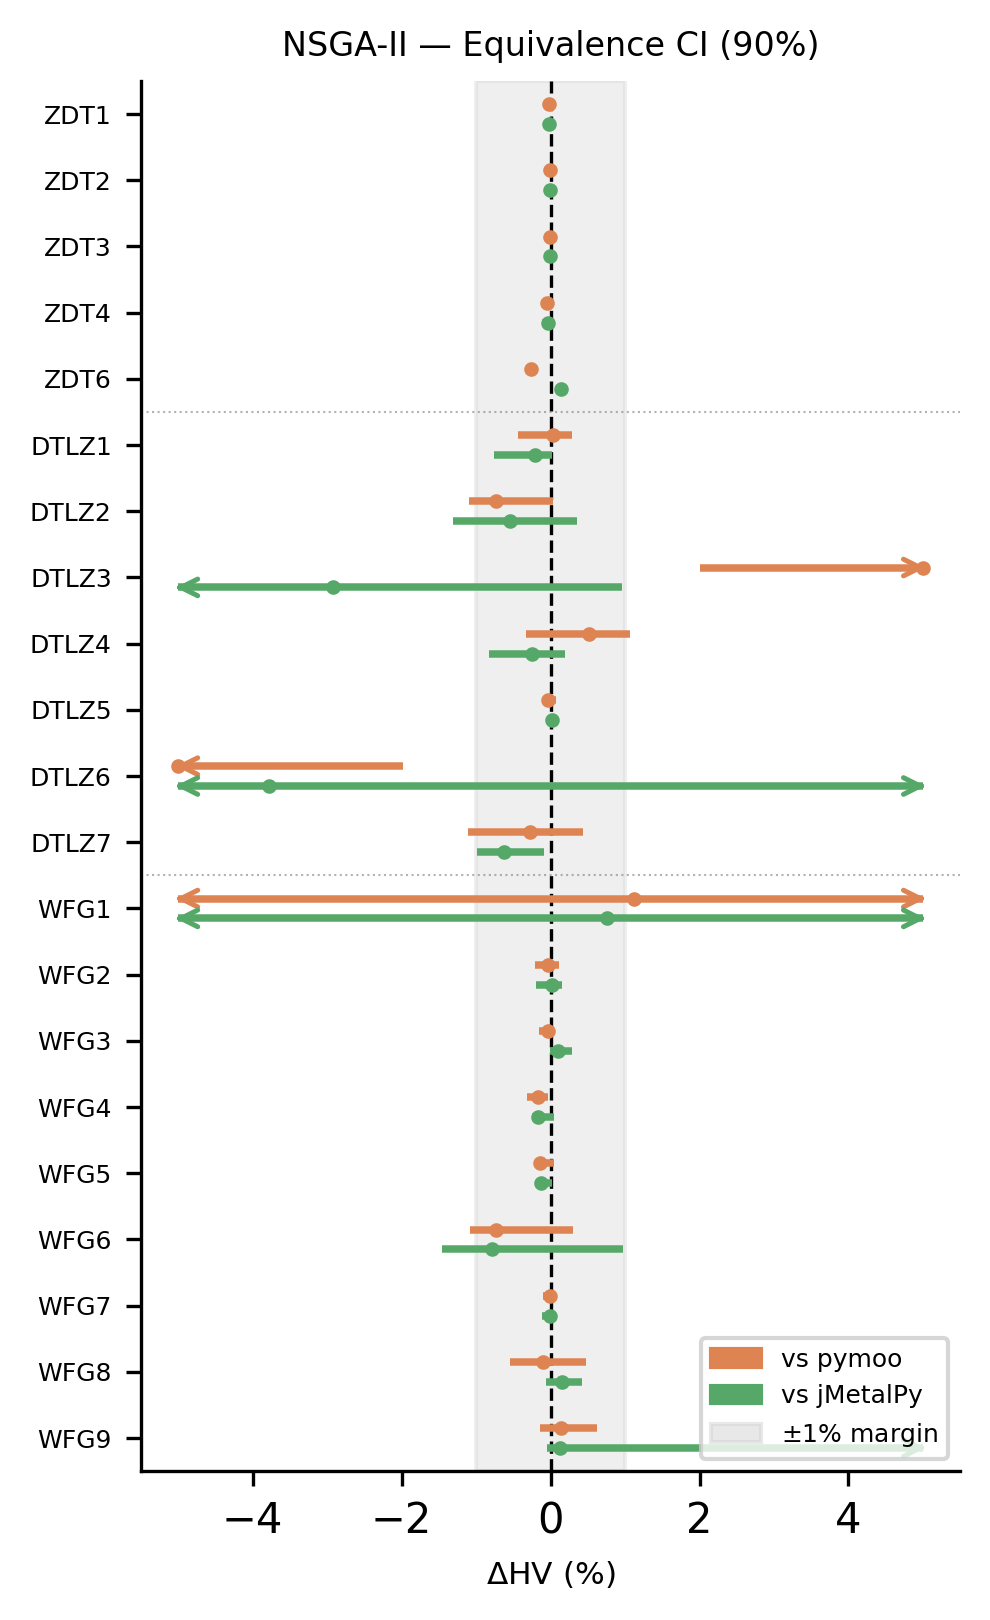
\includegraphics[width=\columnwidth]{figures/forest_ci_nsgaii.png}
  \caption{NSGA-II. Per-problem paired bootstrap 90\% confidence intervals for the relative normalized hypervolume difference $\Delta = (\HV_{\text{\VAMOS}} - \HV_{\text{fw}})/\HV_{\text{fw}}$, reported in percent. The shaded band marks the $\pm 1\%$ equivalence margin; intervals falling entirely within this band indicate statistical equivalence}
  \label{fig:forest_ci_nsgaii}
\end{figure}




\begin{table}[htbp]
\centering
\caption{NSGA-II. Normalized hypervolume comparison with Wilcoxon signed-rank test results (Holm-corrected)}
\label{tab:stats_hypervolume_nsgaii}
\begin{tabular}{lccccc}
\toprule
\textbf{Problem} & \textbf{VAMOS} & \textbf{pymoo} & \textbf{p-value} & \textbf{$\hat{A}_{12}$} & \textbf{Significance} \\
\midrule
dtlz1 & 0.920 & \textbf{0.921} & 1.000 & 0.47 & \xmark \\
dtlz2 & 0.826 & \textbf{0.827} & 1.000 & 0.46 & \xmark \\
dtlz3 & \textbf{0.749} & 0.673 & 0.813 & 0.66 & \xmark \\
dtlz4 & 0.828 & \textbf{0.829} & 1.000 & 0.49 & \xmark \\
dtlz5 & 0.966 & \textbf{0.966} & 1.000 & 0.45 & \xmark \\
dtlz6 & 0.444 & \textbf{0.510} & 1.000 & 0.32 & \xmark \\
dtlz7 & \textbf{0.876} & 0.874 & 1.000 & 0.53 & \xmark \\
wfg1 & 0.353 & \textbf{0.430} & 1.000 & 0.36 & \xmark \\
wfg2 & 1.007 & \textbf{1.007} & 1.000 & 0.37 & \xmark \\
wfg3 & 0.971 & \textbf{0.973} & 1.000 & 0.35 & \xmark \\
wfg4 & 0.956 & \textbf{0.957} & 1.000 & 0.48 & \xmark \\
wfg5 & 0.826 & \textbf{0.826} & 0.513 & 0.32 & \xmark \\
wfg6 & 0.840 & \textbf{0.846} & 1.000 & 0.44 & \xmark \\
wfg7 & 0.963 & \textbf{0.964} & 1.000 & 0.41 & \xmark \\
wfg8 & \textbf{0.745} & 0.745 & 1.000 & 0.54 & \xmark \\
wfg9 & 0.714 & \textbf{0.714} & 1.000 & 0.48 & \xmark \\
zcat1 & 0.983 & \textbf{0.983} & 1.000 & 0.44 & \xmark \\
zcat10 & 0.951 & \textbf{0.951} & 1.000 & 0.43 & \xmark \\
zcat11 & 0.990 & \textbf{0.990} & 1.000 & 0.48 & \xmark \\
zcat12 & 0.989 & \textbf{0.990} & 1.000 & 0.45 & \xmark \\
zcat13 & 1.016 & \textbf{1.016} & 1.000 & 0.47 & \xmark \\
zcat14 & 0.977 & \textbf{0.977} & 1.000 & 0.36 & \xmark \\
zcat15 & 0.989 & \textbf{0.990} & 1.000 & 0.45 & \xmark \\
zcat16 & 0.987 & \textbf{0.988} & 1.000 & 0.40 & \xmark \\
zcat17 & 0.995 & \textbf{0.995} & 1.000 & 0.46 & \xmark \\
zcat18 & \textbf{0.990} & 0.990 & 1.000 & 0.52 & \xmark \\
zcat19 & 0.986 & \textbf{0.986} & 1.000 & 0.42 & \xmark \\
zcat2 & 0.992 & \textbf{0.992} & 1.000 & 0.49 & \xmark \\
zcat20 & \textbf{0.990} & 0.990 & 1.000 & 0.52 & \xmark \\
zcat3 & 0.983 & \textbf{0.983} & 1.000 & 0.37 & \xmark \\
zcat4 & 0.983 & \textbf{0.983} & 1.000 & 0.37 & \xmark \\
zcat5 & 0.995 & \textbf{0.995} & 1.000 & 0.46 & \xmark \\
zcat6 & 0.995 & \textbf{0.995} & 1.000 & 0.46 & \xmark \\
zcat7 & \textbf{0.990} & 0.990 & 1.000 & 0.52 & \xmark \\
zcat8 & 0.971 & \textbf{0.971} & 1.000 & 0.49 & \xmark \\
zcat9 & 0.971 & \textbf{0.971} & 1.000 & 0.49 & \xmark \\
zdt1 & 0.991 & \textbf{0.991} & 1.000 & 0.42 & \xmark \\
zdt2 & 0.982 & \textbf{0.982} & 1.000 & 0.44 & \xmark \\
zdt3 & 0.996 & \textbf{0.996} & 1.000 & 0.55 & \xmark \\
zdt4 & 1.001 & \textbf{1.001} & 1.000 & 0.43 & \xmark \\
zdt6 & 0.982 & \textbf{0.986} & $<$0.0001 & 0.00 & \cmark \\
\bottomrule
\end{tabular}
\end{table}

\begin{table}[htbp]
\centering
\caption{NSGA-II. IGD+ comparison with Wilcoxon signed-rank test results (Holm-corrected). Lower is better}
\label{tab:stats_igd_plus_nsgaii}
\begin{tabular}{lccccc}
\toprule
\textbf{Problem} & \textbf{VAMOS} & \textbf{pymoo} & \textbf{p-value} & \textbf{$\hat{A}_{12}$} & \textbf{Significance} \\
\midrule
dtlz1 & 0.0181 & \textbf{0.0179} & 1.000 & 0.53 &  \xmark \\
dtlz2 & 0.0357 & \textbf{0.0352} & 1.000 & 0.56 &  \xmark \\
dtlz3 & \textbf{0.0518} & 0.0716 & 0.834 & 0.32 &  \xmark \\
dtlz4 & 0.0357 & \textbf{0.0351} & 1.000 & 0.54 &  \xmark \\
dtlz5 & 0.0029 & \textbf{0.0029} & 1.000 & 0.51 &  \xmark \\
dtlz6 & 0.0996 & \textbf{0.0837} & 1.000 & 0.67 &  \xmark \\
dtlz7 & 0.0350 & \textbf{0.0350} & 1.000 & 0.56 &  \xmark \\
wfg1 & 0.7451 & \textbf{0.6949} & 1.000 & 0.65 &  \xmark \\
wfg2 & 0.2162 & \textbf{0.2155} & 1.000 & 0.64 &  \xmark \\
wfg3 & 0.0206 & \textbf{0.0191} & 1.000 & 0.65 &  \xmark \\
wfg4 & 0.0133 & \textbf{0.0128} & 1.000 & 0.53 &  \xmark \\
wfg5 & \textbf{0.0699} & 0.0700 & 1.000 & 0.51 &  \xmark \\
wfg6 & 0.0600 & \textbf{0.0573} & 1.000 & 0.59 &  \xmark \\
wfg7 & 0.0106 & \textbf{0.0103} & 1.000 & 0.58 &  \xmark \\
wfg8 & \textbf{0.1463} & 0.1485 & 1.000 & 0.45 &  \xmark \\
wfg9 & \textbf{0.1263} & 0.1264 & 1.000 & 0.51 &  \xmark \\
zcat1 & 0.0074 & \textbf{0.0073} & 1.000 & 0.58 &  \xmark \\
zcat10 & 0.0033 & \textbf{0.0032} & 1.000 & 0.57 &  \xmark \\
zcat11 & 0.0049 & \textbf{0.0049} & 1.000 & 0.49 &  \xmark \\
zcat12 & 0.0050 & \textbf{0.0049} & 1.000 & 0.52 &  \xmark \\
zcat13 & 0.0038 & \textbf{0.0037} & 1.000 & 0.57 &  \xmark \\
zcat14 & 0.0070 & \textbf{0.0069} & 1.000 & 0.64 &  \xmark \\
zcat15 & 0.0050 & \textbf{0.0050} & 1.000 & 0.52 &  \xmark \\
zcat16 & 0.0048 & \textbf{0.0046} & 1.000 & 0.58 &  \xmark \\
zcat17 & 0.0040 & \textbf{0.0040} & 1.000 & 0.51 &  \xmark \\
zcat18 & \textbf{0.0044} & 0.0044 & 1.000 & 0.51 &  \xmark \\
zcat19 & 0.0062 & \textbf{0.0061} & 1.000 & 0.58 &  \xmark \\
zcat2 & 0.0059 & \textbf{0.0059} & 1.000 & 0.52 &  \xmark \\
zcat20 & \textbf{0.0045} & 0.0045 & 1.000 & 0.52 &  \xmark \\
zcat3 & 0.0074 & \textbf{0.0072} & 1.000 & 0.63 &  \xmark \\
zcat4 & 0.0074 & \textbf{0.0072} & 1.000 & 0.63 &  \xmark \\
zcat5 & 0.0040 & \textbf{0.0040} & 1.000 & 0.53 &  \xmark \\
zcat6 & 0.0027 & \textbf{0.0026} & 1.000 & 0.63 &  \xmark \\
zcat7 & \textbf{0.0044} & 0.0044 & 1.000 & 0.52 &  \xmark \\
zcat8 & 0.0057 & \textbf{0.0056} & 1.000 & 0.51 &  \xmark \\
zcat9 & 0.0057 & \textbf{0.0057} & 1.000 & 0.50 &  \xmark \\
zdt1 & 0.0032 & \textbf{0.0031} & 1.000 & 0.53 &  \xmark \\
zdt2 & 0.0030 & \textbf{0.0030} & 1.000 & 0.53 &  \xmark \\
zdt3 & \textbf{0.0015} & 0.0015 & 1.000 & 0.45 &  \xmark \\
zdt4 & 0.0008 & \textbf{0.0008} & 1.000 & 0.59 &  \xmark \\
zdt6 & 0.0031 & \textbf{0.0024} & $<$0.0001 & 1.00 & \checkmark \\
\bottomrule
\end{tabular}
\end{table}

\begin{table}[htbp]
\centering
\caption{Normalized hypervolume equivalence summary (paired bootstrap 90\% CI; equivalence margin $\pm 1\%$ relative)}
\label{tab:hv_equivalence_summary_nsgaii}
\resizebox{\columnwidth}{!}{%
\begin{tabular}{lccc}
\toprule
\textbf{Framework} & \textbf{Eq.\ problems} & \textbf{Non-inf.\ problems} & \textbf{Median $\Delta$HV (\%)} \\
\midrule
\textit{pymoo} & 37/41 & 38/41 & -0.01 \\
\textit{jMetalPy} & 35/41 & 35/41 & -0.02 \\
\textit{DEAP} & 33/41 & 37/41 & -0.01 \\
\textit{Platypus} & 33/41 & 38/41 & +0.05 \\
\bottomrule
\end{tabular}%
}
\end{table}

\begin{table}[htbp]
\centering
\caption{Robustness summary for normalized hypervolume across seeds (median across problems). ``Near-best'' is defined per problem as HV $\ge 0.99 \cdot \max$ median(HV) among frameworks}
\label{tab:hv_robustness_summary_nsgaii}
\begin{tabular}{lcc}
\toprule
\textbf{Framework} & \textbf{Median IQR(HV)} & \textbf{Median \% seeds near-best} \\
\midrule
VAMOS & 0.001 & 100.0 \\
\textit{pymoo} & 0.001 & 100.0 \\
\textit{jMetalPy} & 0.002 & 100.0 \\
\textit{DEAP} & 0.001 & 100.0 \\
\textit{Platypus} & 0.001 & 100.0 \\
\bottomrule
\end{tabular}
\end{table}

\begin{figure}[htbp]
  \centering
  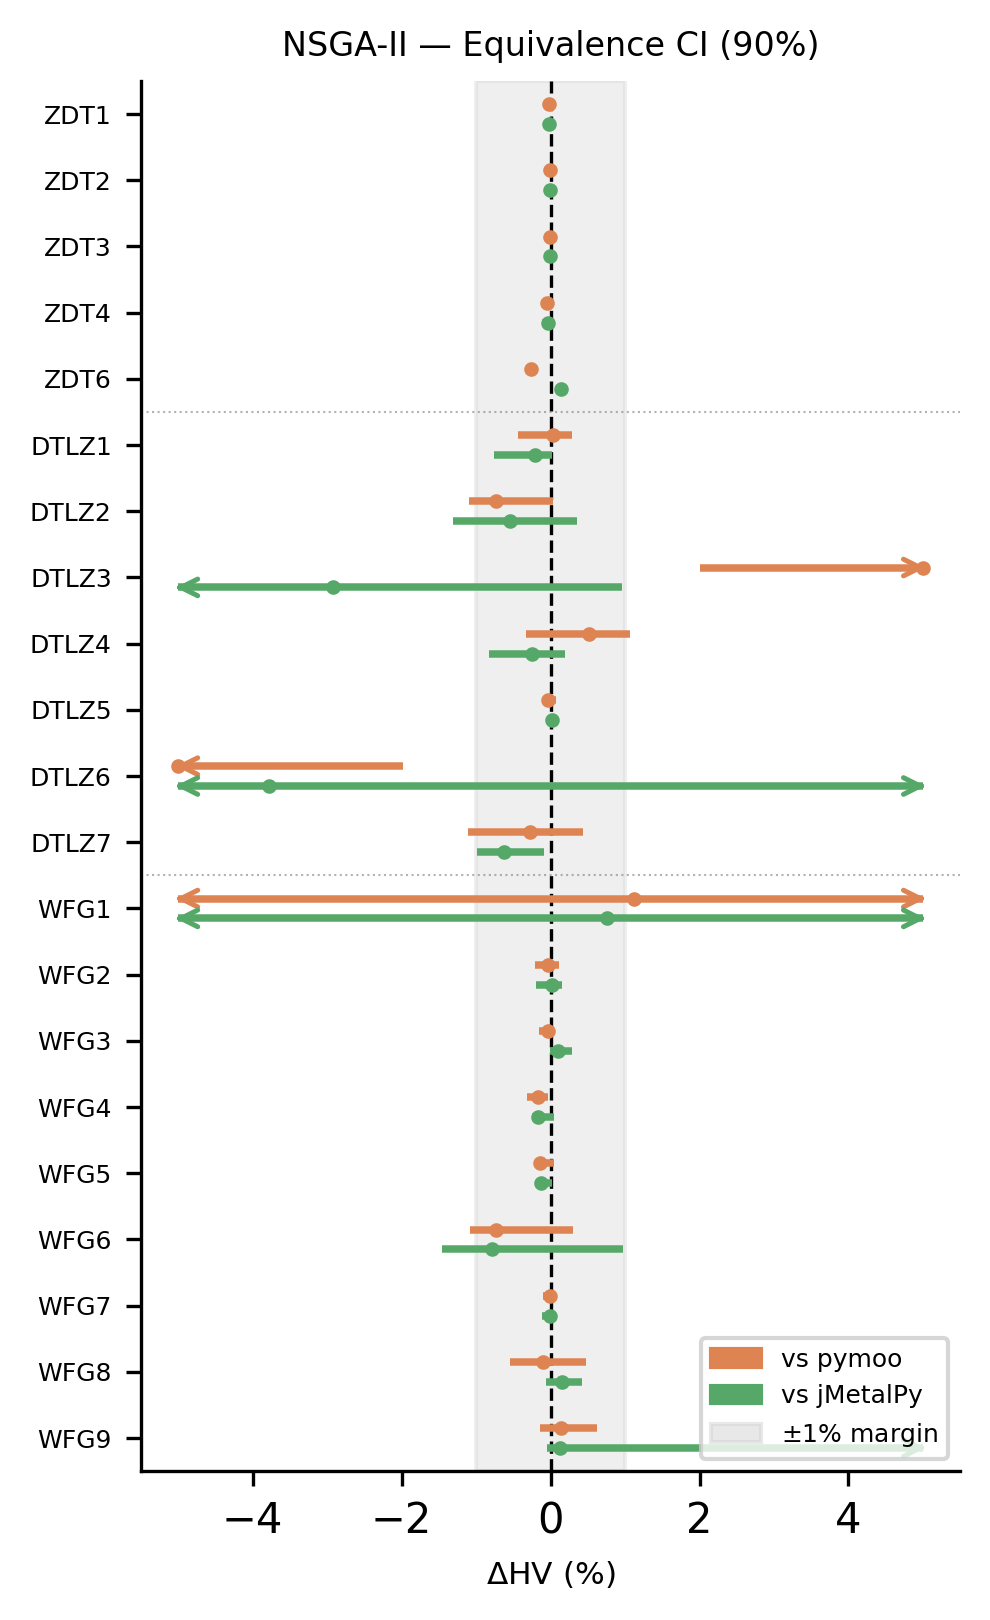
\includegraphics[width=\columnwidth]{figures/forest_ci_nsgaii.png}
  \caption{NSGA-II. Per-problem paired bootstrap 90\% confidence intervals for the relative normalized hypervolume difference $\Delta = (\HV_{\text{\VAMOS}} - \HV_{\text{fw}})/\HV_{\text{fw}}$, reported in percent. The shaded band marks the $\pm 1\%$ equivalence margin; intervals falling entirely within this band indicate statistical equivalence}
  \label{fig:forest_ci_nsgaii}
\end{figure}




\begin{table}[htbp]
\centering
\caption{NSGA-II. Normalized hypervolume comparison with Wilcoxon signed-rank test results (Holm-corrected)}
\label{tab:stats_hypervolume_nsgaii}
\begin{tabular}{lccccc}
\toprule
\textbf{Problem} & \textbf{VAMOS} & \textbf{pymoo} & \textbf{p-value} & \textbf{$\hat{A}_{12}$} & \textbf{Significance} \\
\midrule
dtlz1 & 0.920 & \textbf{0.921} & 1.000 & 0.47 & \xmark \\
dtlz2 & 0.826 & \textbf{0.827} & 1.000 & 0.46 & \xmark \\
dtlz3 & \textbf{0.749} & 0.673 & 0.813 & 0.66 & \xmark \\
dtlz4 & 0.828 & \textbf{0.829} & 1.000 & 0.49 & \xmark \\
dtlz5 & 0.966 & \textbf{0.966} & 1.000 & 0.45 & \xmark \\
dtlz6 & 0.444 & \textbf{0.510} & 1.000 & 0.32 & \xmark \\
dtlz7 & \textbf{0.876} & 0.874 & 1.000 & 0.53 & \xmark \\
wfg1 & 0.353 & \textbf{0.430} & 1.000 & 0.36 & \xmark \\
wfg2 & 1.007 & \textbf{1.007} & 1.000 & 0.37 & \xmark \\
wfg3 & 0.971 & \textbf{0.973} & 1.000 & 0.35 & \xmark \\
wfg4 & 0.956 & \textbf{0.957} & 1.000 & 0.48 & \xmark \\
wfg5 & 0.826 & \textbf{0.826} & 0.513 & 0.32 & \xmark \\
wfg6 & 0.840 & \textbf{0.846} & 1.000 & 0.44 & \xmark \\
wfg7 & 0.963 & \textbf{0.964} & 1.000 & 0.41 & \xmark \\
wfg8 & \textbf{0.745} & 0.745 & 1.000 & 0.54 & \xmark \\
wfg9 & 0.714 & \textbf{0.714} & 1.000 & 0.48 & \xmark \\
zcat1 & 0.983 & \textbf{0.983} & 1.000 & 0.44 & \xmark \\
zcat10 & 0.951 & \textbf{0.951} & 1.000 & 0.43 & \xmark \\
zcat11 & 0.990 & \textbf{0.990} & 1.000 & 0.48 & \xmark \\
zcat12 & 0.989 & \textbf{0.990} & 1.000 & 0.45 & \xmark \\
zcat13 & 1.016 & \textbf{1.016} & 1.000 & 0.47 & \xmark \\
zcat14 & 0.977 & \textbf{0.977} & 1.000 & 0.36 & \xmark \\
zcat15 & 0.989 & \textbf{0.990} & 1.000 & 0.45 & \xmark \\
zcat16 & 0.987 & \textbf{0.988} & 1.000 & 0.40 & \xmark \\
zcat17 & 0.995 & \textbf{0.995} & 1.000 & 0.46 & \xmark \\
zcat18 & \textbf{0.990} & 0.990 & 1.000 & 0.52 & \xmark \\
zcat19 & 0.986 & \textbf{0.986} & 1.000 & 0.42 & \xmark \\
zcat2 & 0.992 & \textbf{0.992} & 1.000 & 0.49 & \xmark \\
zcat20 & \textbf{0.990} & 0.990 & 1.000 & 0.52 & \xmark \\
zcat3 & 0.983 & \textbf{0.983} & 1.000 & 0.37 & \xmark \\
zcat4 & 0.983 & \textbf{0.983} & 1.000 & 0.37 & \xmark \\
zcat5 & 0.995 & \textbf{0.995} & 1.000 & 0.46 & \xmark \\
zcat6 & 0.995 & \textbf{0.995} & 1.000 & 0.46 & \xmark \\
zcat7 & \textbf{0.990} & 0.990 & 1.000 & 0.52 & \xmark \\
zcat8 & 0.971 & \textbf{0.971} & 1.000 & 0.49 & \xmark \\
zcat9 & 0.971 & \textbf{0.971} & 1.000 & 0.49 & \xmark \\
zdt1 & 0.991 & \textbf{0.991} & 1.000 & 0.42 & \xmark \\
zdt2 & 0.982 & \textbf{0.982} & 1.000 & 0.44 & \xmark \\
zdt3 & 0.996 & \textbf{0.996} & 1.000 & 0.55 & \xmark \\
zdt4 & 1.001 & \textbf{1.001} & 1.000 & 0.43 & \xmark \\
zdt6 & 0.982 & \textbf{0.986} & $<$0.0001 & 0.00 & \cmark \\
\bottomrule
\end{tabular}
\end{table}

\begin{table}[htbp]
\centering
\caption{NSGA-II. IGD+ comparison with Wilcoxon signed-rank test results (Holm-corrected). Lower is better}
\label{tab:stats_igd_plus_nsgaii}
\begin{tabular}{lccccc}
\toprule
\textbf{Problem} & \textbf{VAMOS} & \textbf{pymoo} & \textbf{p-value} & \textbf{$\hat{A}_{12}$} & \textbf{Significance} \\
\midrule
dtlz1 & 0.0181 & \textbf{0.0179} & 1.000 & 0.53 &  \xmark \\
dtlz2 & 0.0357 & \textbf{0.0352} & 1.000 & 0.56 &  \xmark \\
dtlz3 & \textbf{0.0518} & 0.0716 & 0.834 & 0.32 &  \xmark \\
dtlz4 & 0.0357 & \textbf{0.0351} & 1.000 & 0.54 &  \xmark \\
dtlz5 & 0.0029 & \textbf{0.0029} & 1.000 & 0.51 &  \xmark \\
dtlz6 & 0.0996 & \textbf{0.0837} & 1.000 & 0.67 &  \xmark \\
dtlz7 & 0.0350 & \textbf{0.0350} & 1.000 & 0.56 &  \xmark \\
wfg1 & 0.7451 & \textbf{0.6949} & 1.000 & 0.65 &  \xmark \\
wfg2 & 0.2162 & \textbf{0.2155} & 1.000 & 0.64 &  \xmark \\
wfg3 & 0.0206 & \textbf{0.0191} & 1.000 & 0.65 &  \xmark \\
wfg4 & 0.0133 & \textbf{0.0128} & 1.000 & 0.53 &  \xmark \\
wfg5 & \textbf{0.0699} & 0.0700 & 1.000 & 0.51 &  \xmark \\
wfg6 & 0.0600 & \textbf{0.0573} & 1.000 & 0.59 &  \xmark \\
wfg7 & 0.0106 & \textbf{0.0103} & 1.000 & 0.58 &  \xmark \\
wfg8 & \textbf{0.1463} & 0.1485 & 1.000 & 0.45 &  \xmark \\
wfg9 & \textbf{0.1263} & 0.1264 & 1.000 & 0.51 &  \xmark \\
zcat1 & 0.0074 & \textbf{0.0073} & 1.000 & 0.58 &  \xmark \\
zcat10 & 0.0033 & \textbf{0.0032} & 1.000 & 0.57 &  \xmark \\
zcat11 & 0.0049 & \textbf{0.0049} & 1.000 & 0.49 &  \xmark \\
zcat12 & 0.0050 & \textbf{0.0049} & 1.000 & 0.52 &  \xmark \\
zcat13 & 0.0038 & \textbf{0.0037} & 1.000 & 0.57 &  \xmark \\
zcat14 & 0.0070 & \textbf{0.0069} & 1.000 & 0.64 &  \xmark \\
zcat15 & 0.0050 & \textbf{0.0050} & 1.000 & 0.52 &  \xmark \\
zcat16 & 0.0048 & \textbf{0.0046} & 1.000 & 0.58 &  \xmark \\
zcat17 & 0.0040 & \textbf{0.0040} & 1.000 & 0.51 &  \xmark \\
zcat18 & \textbf{0.0044} & 0.0044 & 1.000 & 0.51 &  \xmark \\
zcat19 & 0.0062 & \textbf{0.0061} & 1.000 & 0.58 &  \xmark \\
zcat2 & 0.0059 & \textbf{0.0059} & 1.000 & 0.52 &  \xmark \\
zcat20 & \textbf{0.0045} & 0.0045 & 1.000 & 0.52 &  \xmark \\
zcat3 & 0.0074 & \textbf{0.0072} & 1.000 & 0.63 &  \xmark \\
zcat4 & 0.0074 & \textbf{0.0072} & 1.000 & 0.63 &  \xmark \\
zcat5 & 0.0040 & \textbf{0.0040} & 1.000 & 0.53 &  \xmark \\
zcat6 & 0.0027 & \textbf{0.0026} & 1.000 & 0.63 &  \xmark \\
zcat7 & \textbf{0.0044} & 0.0044 & 1.000 & 0.52 &  \xmark \\
zcat8 & 0.0057 & \textbf{0.0056} & 1.000 & 0.51 &  \xmark \\
zcat9 & 0.0057 & \textbf{0.0057} & 1.000 & 0.50 &  \xmark \\
zdt1 & 0.0032 & \textbf{0.0031} & 1.000 & 0.53 &  \xmark \\
zdt2 & 0.0030 & \textbf{0.0030} & 1.000 & 0.53 &  \xmark \\
zdt3 & \textbf{0.0015} & 0.0015 & 1.000 & 0.45 &  \xmark \\
zdt4 & 0.0008 & \textbf{0.0008} & 1.000 & 0.59 &  \xmark \\
zdt6 & 0.0031 & \textbf{0.0024} & $<$0.0001 & 1.00 & \checkmark \\
\bottomrule
\end{tabular}
\end{table}

\begin{table}[htbp]
\centering
\caption{Normalized hypervolume equivalence summary (paired bootstrap 90\% CI; equivalence margin $\pm 1\%$ relative)}
\label{tab:hv_equivalence_summary_nsgaii}
\resizebox{\columnwidth}{!}{%
\begin{tabular}{lccc}
\toprule
\textbf{Framework} & \textbf{Eq.\ problems} & \textbf{Non-inf.\ problems} & \textbf{Median $\Delta$HV (\%)} \\
\midrule
\textit{pymoo} & 37/41 & 38/41 & -0.01 \\
\textit{jMetalPy} & 35/41 & 35/41 & -0.02 \\
\textit{DEAP} & 33/41 & 37/41 & -0.01 \\
\textit{Platypus} & 33/41 & 38/41 & +0.05 \\
\bottomrule
\end{tabular}%
}
\end{table}

\begin{table}[htbp]
\centering
\caption{Robustness summary for normalized hypervolume across seeds (median across problems). ``Near-best'' is defined per problem as HV $\ge 0.99 \cdot \max$ median(HV) among frameworks}
\label{tab:hv_robustness_summary_nsgaii}
\begin{tabular}{lcc}
\toprule
\textbf{Framework} & \textbf{Median IQR(HV)} & \textbf{Median \% seeds near-best} \\
\midrule
VAMOS & 0.001 & 100.0 \\
\textit{pymoo} & 0.001 & 100.0 \\
\textit{jMetalPy} & 0.002 & 100.0 \\
\textit{DEAP} & 0.001 & 100.0 \\
\textit{Platypus} & 0.001 & 100.0 \\
\bottomrule
\end{tabular}
\end{table}

\begin{figure}[htbp]
  \centering
  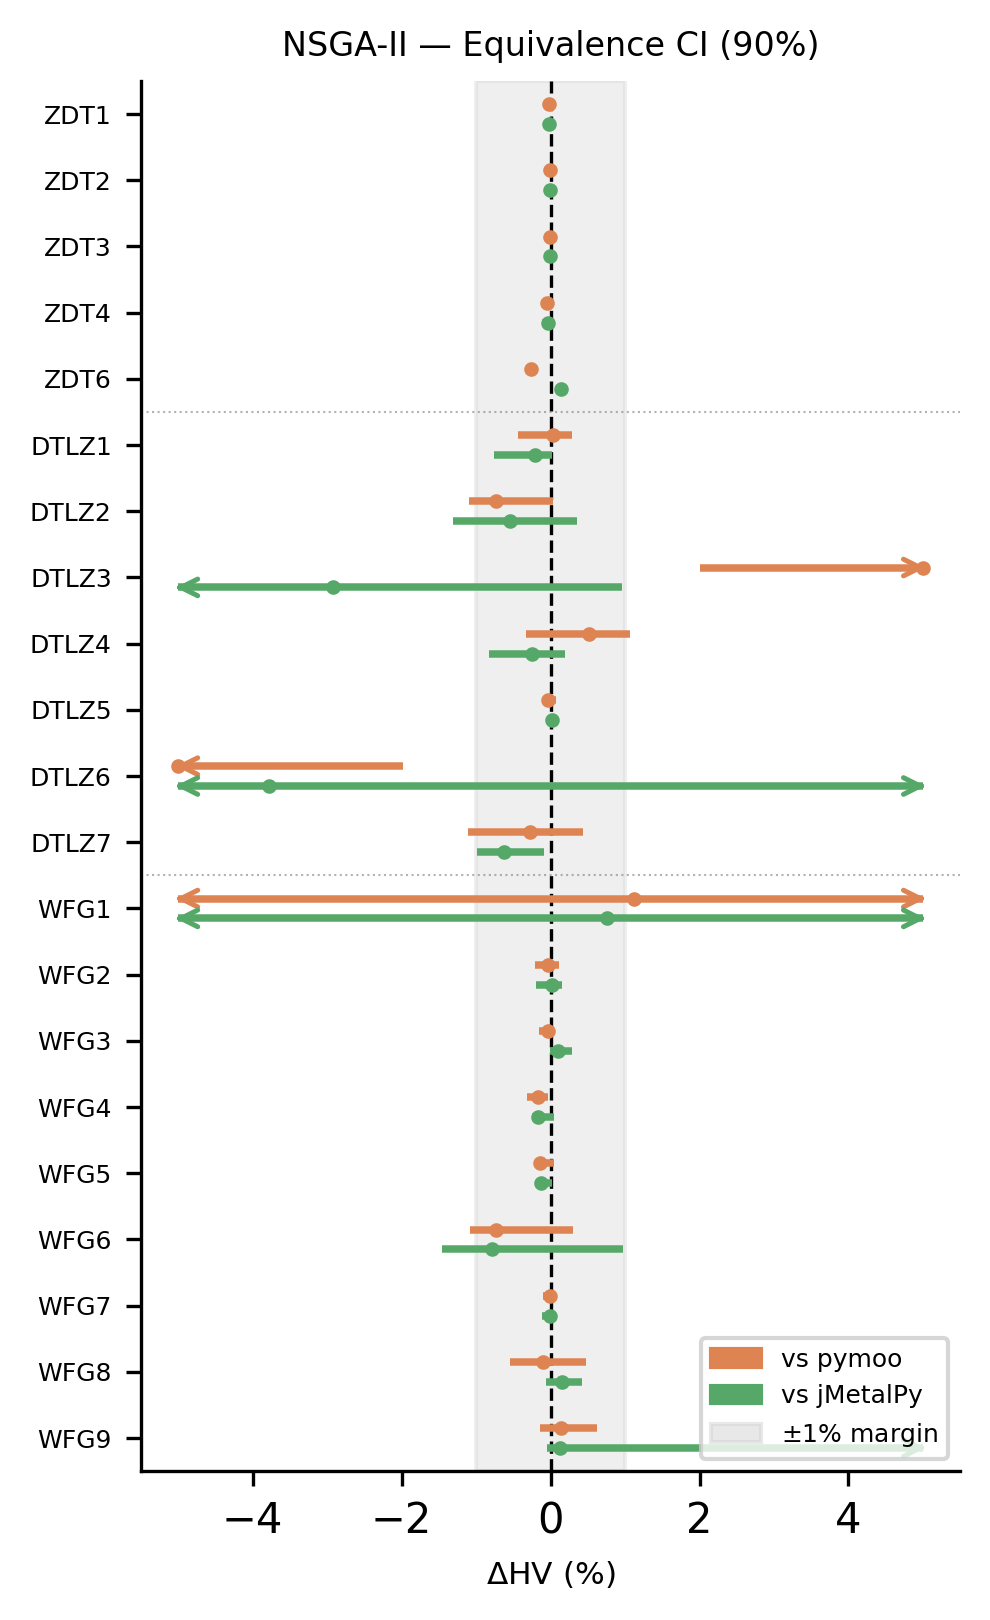
\includegraphics[width=\columnwidth]{figures/forest_ci_nsgaii.png}
  \caption{NSGA-II. Per-problem paired bootstrap 90\% confidence intervals for the relative normalized hypervolume difference $\Delta = (\HV_{\text{\VAMOS}} - \HV_{\text{fw}})/\HV_{\text{fw}}$, reported in percent. The shaded band marks the $\pm 1\%$ equivalence margin; intervals falling entirely within this band indicate statistical equivalence}
  \label{fig:forest_ci_nsgaii}
\end{figure}

\endgroup

\section{Reference fronts and detailed benchmark results}
\label{app:detailed}
%==============================================================================

The repository includes dense reference Pareto fronts for all benchmark problems used for normalized hypervolume computation. These fronts are generated analytically when closed forms are available (ZDT and most DTLZ problems) and by dense sampling followed by non-dominated filtering for cases where the Pareto front is disconnected or defined implicitly (DTLZ7 and WFG). For WFG2 we use a higher sampling density to stabilize HV normalization.

Fig.~\ref{fig:runtime_heatmap} presents per-problem median runtimes as a dual-panel heatmap. The left panel compares VAMOS backends (Numba, MooCore, NumPy); the right panel compares VAMOS against pymoo and jMetalPy. Color intensity indicates runtime on a logarithmic scale, with annotated values in each cell and bold values marking the fastest per problem.

\begin{figure*}[htbp]
  \centering
  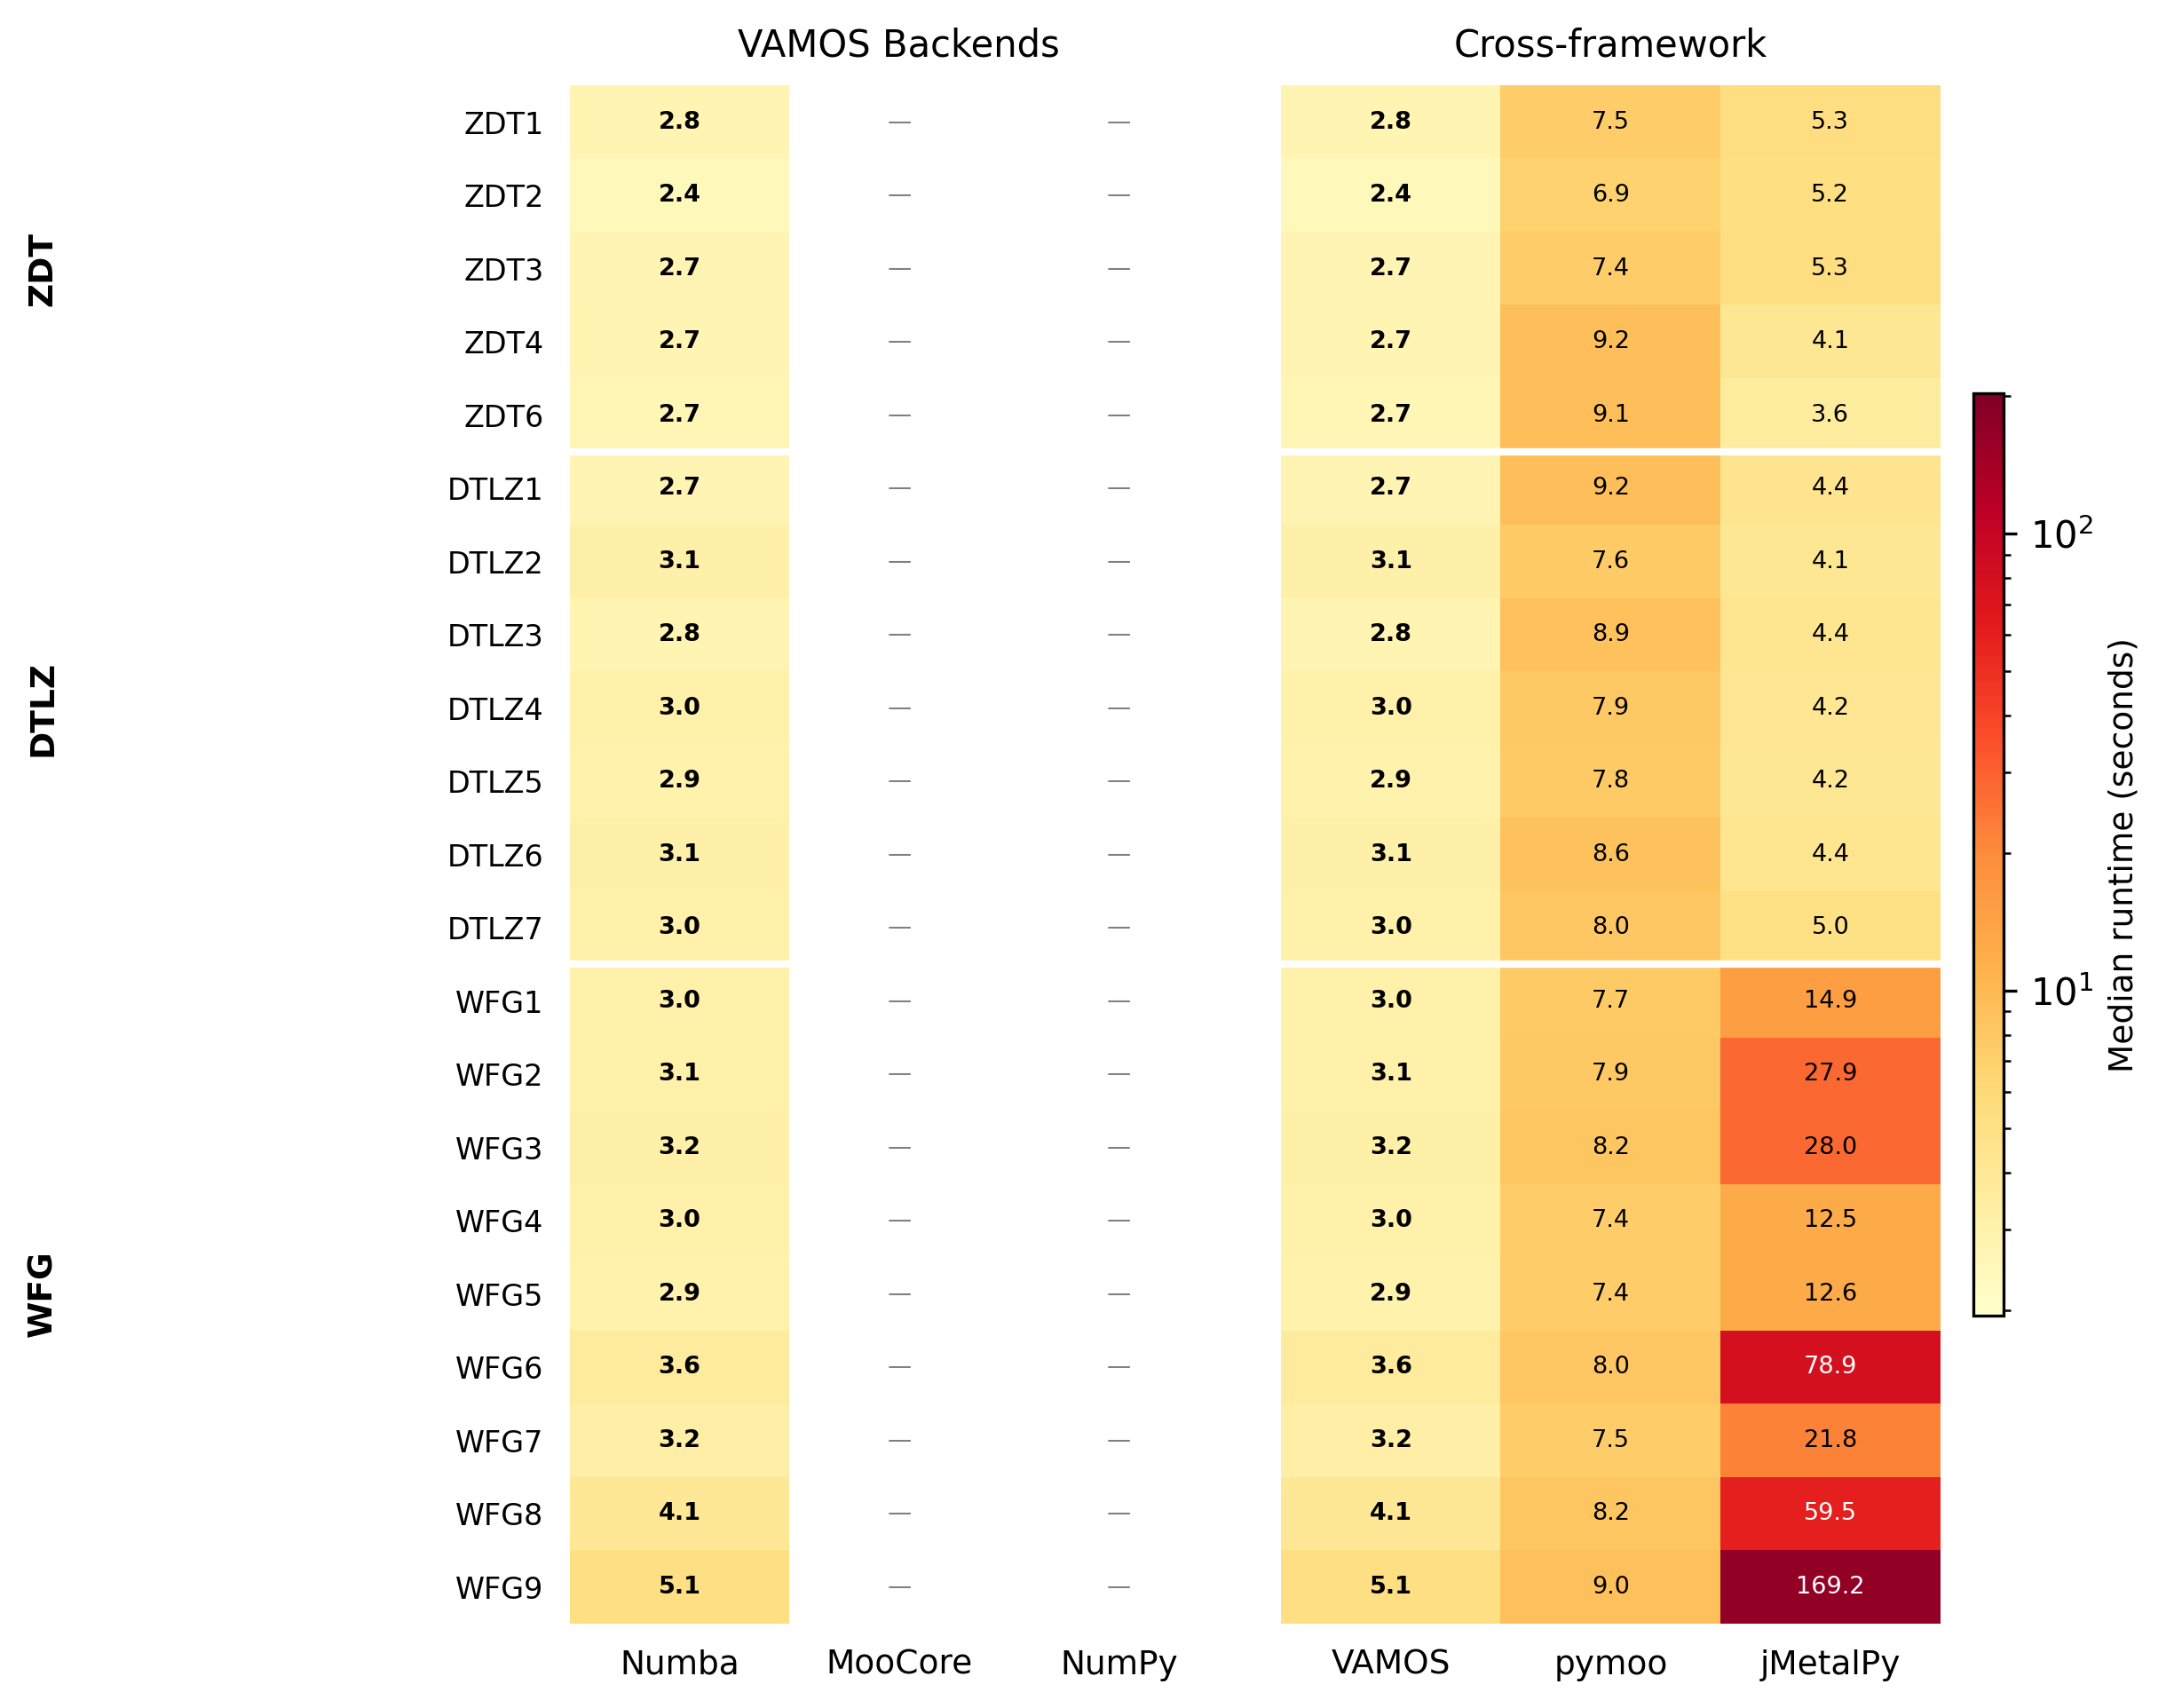
\includegraphics[width=0.95\textwidth]{figures/runtime_heatmap.png}
  \caption{Per-problem median runtime (seconds) for VAMOS backends (left) and cross-framework comparison (right). Color scale is logarithmic; bold values indicate the fastest in each row. Problems are grouped by family (ZDT, DTLZ, WFG).}
  \label{fig:runtime_heatmap}
\end{figure*}

%==============================================================================
\section{Statistical analysis for SMS-EMOA and MOEA/D}
\label{app:stats}
%==============================================================================

Tables in this appendix report Wilcoxon signed-rank tests, bootstrap equivalence analyses, and robustness summaries for SMS-EMOA and MOEA/D, following the same methodology as the Statistical Analysis section of the main paper.

\subsection{SMS-EMOA}

Tables~\ref{tab:stats_hypervolume_smsemoa}--\ref{tab:hv_robustness_summary_smsemoa} present per-problem Wilcoxon tests, equivalence summaries, and robustness summaries for SMS-EMOA. Fig.~\ref{fig:forest_ci_smsemoa} visualizes per-problem bootstrap confidence intervals.

\begingroup
\setlength{\tabcolsep}{2pt}
% Auto-generated by paper/05_run_statistical_tests.py

% Algorithm: SMS-EMOA (smsemoa)

% Source CSV: C:\Users\nicor\Desktop\VAMOS\experiments\benchmark_paper_smsemoa.csv

%

% Include from main.tex with: % Auto-generated by paper/05_run_statistical_tests.py

% Algorithm: SMS-EMOA (smsemoa)

% Source CSV: C:\Users\nicor\Desktop\VAMOS\experiments\benchmark_paper_smsemoa.csv

%

% Include from main.tex with: % Auto-generated by paper/05_run_statistical_tests.py

% Algorithm: SMS-EMOA (smsemoa)

% Source CSV: C:\Users\nicor\Desktop\VAMOS\experiments\benchmark_paper_smsemoa.csv

%

% Include from main.tex with: \input{stats_smsemoa.tex}



\begin{table}[htbp]
\centering
\caption{SMS-EMOA. Normalized hypervolume comparison with Wilcoxon signed-rank test results (Holm-corrected)}
\label{tab:stats_hypervolume_smsemoa}
\begin{tabular}{lrrrrl}
\toprule
\textbf{Problem} & \textbf{VAMOS (numba)} & \textbf{pymoo} & \textbf{p-value} & \textbf{$\hat{A}_{12}$} & \textbf{Sig.} \\
\midrule
zdt1 & 0.993 & \textbf{0.993} & 1.000 & 0.46 &  \\
zdt2 & 0.987 & \textbf{0.987} & 1.000 & 0.43 &  \\
zdt3 & \textbf{0.997} & 0.997 & 1.000 & 0.50 &  \\
zdt4 & \textbf{1.004} & 1.004 & 1.000 & 0.57 &  \\
zdt6 & \textbf{0.989} & 0.989 & 1.000 & 0.58 &  \\
dtlz1 & \textbf{0.959} & 0.959 & 1.000 & 0.56 &  \\
dtlz2 & \textbf{0.933} & 0.933 & 1.000 & 0.53 &  \\
dtlz3 & \textbf{0.903} & 0.903 & 1.000 & 0.50 &  \\
dtlz4 & \textbf{0.933} & 0.712 & 0.730 & 0.60 &  \\
dtlz5 & 0.978 & \textbf{0.978} & 0.002 & 0.21 & $\checkmark$ \\
dtlz6 & 0.553 & \textbf{0.566} & 1.000 & 0.44 &  \\
dtlz7 & 0.949 & \textbf{0.950} & 0.152 & 0.17 &  \\
wfg1 & 0.244 & \textbf{0.258} & 1.000 & 0.46 &  \\
wfg2 & 1.009 & \textbf{1.010} & 1.000 & 0.49 &  \\
wfg3 & 0.983 & \textbf{0.983} & 1.000 & 0.43 &  \\
wfg4 & \textbf{0.980} & 0.980 & 1.000 & 0.56 &  \\
wfg5 & 0.836 & \textbf{0.836} & 1.000 & 0.52 &  \\
wfg6 & 0.856 & \textbf{0.858} & 1.000 & 0.51 &  \\
wfg7 & 0.982 & \textbf{0.982} & 1.000 & 0.45 &  \\
wfg8 & 0.774 & \textbf{0.775} & 1.000 & 0.44 &  \\
wfg9 & \textbf{0.963} & 0.961 & 1.000 & 0.53 &  \\
\bottomrule
\end{tabular}
\end{table}

\begin{table}[htbp]
\centering
\caption{SMS-EMOA. IGD+ comparison with Wilcoxon signed-rank test results (Holm-corrected). Lower is better}
\label{tab:stats_igd_plus_smsemoa}
\begin{tabular}{lrrrrl}
\toprule
\textbf{Problem} & \textbf{VAMOS (numba)} & \textbf{pymoo} & \textbf{p-value} & \textbf{$\hat{A}_{12}$} & \textbf{Sig.} \\
\midrule
zdt1 & 0.0023 & \textbf{0.0023} & 1.000 & 0.52 &  \\
zdt2 & \textbf{0.0022} & 0.0022 & 1.000 & 0.52 &  \\
zdt3 & \textbf{0.0010} & 0.0010 & 1.000 & 0.47 &  \\
zdt4 & \textbf{0.0003} & 0.0003 & 1.000 & 0.47 &  \\
zdt6 & \textbf{0.0019} & 0.0019 & 1.000 & 0.43 &  \\
dtlz1 & \textbf{0.0134} & 0.0134 & 1.000 & 0.47 &  \\
dtlz2 & \textbf{0.0183} & 0.0184 & 1.000 & 0.45 &  \\
dtlz3 & 0.0254 & \textbf{0.0252} & 1.000 & 0.51 &  \\
dtlz4 & \textbf{0.0186} & 0.1090 & 1.000 & 0.50 &  \\
dtlz5 & 0.0017 & \textbf{0.0017} & 1.000 & 0.57 &  \\
dtlz6 & 0.0877 & \textbf{0.0852} & 1.000 & 0.56 &  \\
dtlz7 & 0.0221 & \textbf{0.0217} & 0.305 & 0.79 &  \\
wfg1 & 0.8724 & \textbf{0.8573} & 1.000 & 0.53 &  \\
wfg2 & 0.2140 & \textbf{0.2138} & 1.000 & 0.52 &  \\
wfg3 & 0.0118 & \textbf{0.0115} & 1.000 & 0.57 &  \\
wfg4 & \textbf{0.0062} & 0.0062 & 1.000 & 0.51 &  \\
wfg5 & 0.0682 & \textbf{0.0681} & 1.000 & 0.63 &  \\
wfg6 & 0.0560 & \textbf{0.0552} & 1.000 & 0.46 &  \\
wfg7 & 0.0053 & \textbf{0.0053} & 1.000 & 0.54 &  \\
wfg8 & 0.1394 & \textbf{0.1388} & 1.000 & 0.50 &  \\
wfg9 & \textbf{0.0179} & 0.0218 & 1.000 & 0.38 &  \\
\bottomrule
\end{tabular}
\end{table}

\begin{table}[htbp]
\centering
\caption{Normalized hypervolume equivalence summary (paired bootstrap 90\% CI; equivalence margin $\pm 1\%$ relative). Generated by \texttt{paper/05\_run\_statistical\_tests.py}}
\label{tab:hv_equivalence_summary_smsemoa}
\begin{tabular}{lrrr}
\toprule
\textbf{Framework} & \textbf{Eq.\ problems} & \textbf{Non-inf.\ problems} & \textbf{Median $\Delta$HV (\%)} \\
\midrule
pymoo & 16/21 & 19/21 & +0.00 \\
jMetalPy & 15/21 & 18/21 & +0.00 \\
\bottomrule
\end{tabular}
\end{table}

\begin{table}[htbp]
\centering
\caption{Robustness summary for normalized hypervolume across seeds (median across problems). ``Near-best'' is defined per problem as HV $\ge 0.99 \cdot \max$ median(HV) among frameworks. Generated by \texttt{paper/05\_run\_statistical\_tests.py}}
\label{tab:hv_robustness_summary_smsemoa}
\begin{tabular}{lrr}
\toprule
\textbf{Framework} & \textbf{Median IQR(HV)} & \textbf{Median \% seeds near-best} \\
\midrule
VAMOS (numba) & 0.001 & 100.0 \\
pymoo & 0.001 & 100.0 \\
jMetalPy & 0.001 & 100.0 \\
\bottomrule
\end{tabular}
\end{table}

\begin{table*}[htbp]
\tiny
\centering
\caption{Per-problem paired bootstrap 90\% confidence intervals (CI) for the relative normalized hypervolume difference $\Delta = (\HV_{\VAMOS} - \HV_{\text{fw}})/\HV_{\text{fw}}$, reported in percent. Equivalence margin is $\pm 1\%$. Generated by \texttt{paper/05\_run\_statistical\_tests.py}}
\label{tab:hv_equivalence_ci_smsemoa}
\begin{tabular}{lrr}
\toprule
\textbf{Problem} & \textbf{pymoo CI} & \textbf{jMetalPy CI} \\
\midrule
dtlz1 & $[-0.02,+0.02]$ & $[-0.01,+0.01]$ \\
dtlz2 & $[-0.01,+0.01]$ & $[-0.00,+0.01]$ \\
dtlz3 & $[-0.82,+1.09]$ & $[-0.51,+1.46]$ \\
dtlz4 & $[+0.00,+0.01]$ & $[-0.00,+5.29]$ \\
dtlz5 & $[-0.06,-0.01]$ & $[-0.01,+0.02]$ \\
dtlz6 & $[-16.20,+4.60]$ & $[-14.35,-0.44]$ \\
dtlz7 & $[-0.17,-0.09]$ & $[-0.07,+0.08]$ \\
wfg1 & $[-16.45,+9.80]$ & $[-11.19,+5.04]$ \\
wfg2 & $[-0.12,+0.08]$ & $[-0.20,+0.16]$ \\
wfg3 & $[-0.16,+0.05]$ & $[-0.10,+0.05]$ \\
wfg4 & $[-0.01,+0.03]$ & $[-0.07,+0.06]$ \\
wfg5 & $[-0.01,+0.01]$ & $[-0.00,+0.01]$ \\
wfg6 & $[-0.31,+1.38]$ & $[-1.35,+0.87]$ \\
wfg7 & $[-0.03,+0.01]$ & $[-0.03,+0.03]$ \\
wfg8 & $[-0.25,+0.19]$ & $[-0.43,+0.10]$ \\
wfg9 & $[-0.22,+1.17]$ & $[+0.26,+16.50]$ \\
zdt1 & $[-0.00,+0.00]$ & $[-0.00,+0.00]$ \\
zdt2 & $[-0.00,+0.00]$ & $[-0.00,+0.00]$ \\
zdt3 & $[-0.00,+0.00]$ & $[-0.00,+0.00]$ \\
zdt4 & $[-0.01,+0.04]$ & $[-0.05,-0.00]$ \\
zdt6 & $[-0.00,+0.03]$ & $[-0.02,-0.01]$ \\
\bottomrule
\end{tabular}
\end{table*}




\begin{table}[htbp]
\centering
\caption{SMS-EMOA. Normalized hypervolume comparison with Wilcoxon signed-rank test results (Holm-corrected)}
\label{tab:stats_hypervolume_smsemoa}
\begin{tabular}{lrrrrl}
\toprule
\textbf{Problem} & \textbf{VAMOS (numba)} & \textbf{pymoo} & \textbf{p-value} & \textbf{$\hat{A}_{12}$} & \textbf{Sig.} \\
\midrule
zdt1 & 0.993 & \textbf{0.993} & 1.000 & 0.46 &  \\
zdt2 & 0.987 & \textbf{0.987} & 1.000 & 0.43 &  \\
zdt3 & \textbf{0.997} & 0.997 & 1.000 & 0.50 &  \\
zdt4 & \textbf{1.004} & 1.004 & 1.000 & 0.57 &  \\
zdt6 & \textbf{0.989} & 0.989 & 1.000 & 0.58 &  \\
dtlz1 & \textbf{0.959} & 0.959 & 1.000 & 0.56 &  \\
dtlz2 & \textbf{0.933} & 0.933 & 1.000 & 0.53 &  \\
dtlz3 & \textbf{0.903} & 0.903 & 1.000 & 0.50 &  \\
dtlz4 & \textbf{0.933} & 0.712 & 0.730 & 0.60 &  \\
dtlz5 & 0.978 & \textbf{0.978} & 0.002 & 0.21 & $\checkmark$ \\
dtlz6 & 0.553 & \textbf{0.566} & 1.000 & 0.44 &  \\
dtlz7 & 0.949 & \textbf{0.950} & 0.152 & 0.17 &  \\
wfg1 & 0.244 & \textbf{0.258} & 1.000 & 0.46 &  \\
wfg2 & 1.009 & \textbf{1.010} & 1.000 & 0.49 &  \\
wfg3 & 0.983 & \textbf{0.983} & 1.000 & 0.43 &  \\
wfg4 & \textbf{0.980} & 0.980 & 1.000 & 0.56 &  \\
wfg5 & 0.836 & \textbf{0.836} & 1.000 & 0.52 &  \\
wfg6 & 0.856 & \textbf{0.858} & 1.000 & 0.51 &  \\
wfg7 & 0.982 & \textbf{0.982} & 1.000 & 0.45 &  \\
wfg8 & 0.774 & \textbf{0.775} & 1.000 & 0.44 &  \\
wfg9 & \textbf{0.963} & 0.961 & 1.000 & 0.53 &  \\
\bottomrule
\end{tabular}
\end{table}

\begin{table}[htbp]
\centering
\caption{SMS-EMOA. IGD+ comparison with Wilcoxon signed-rank test results (Holm-corrected). Lower is better}
\label{tab:stats_igd_plus_smsemoa}
\begin{tabular}{lrrrrl}
\toprule
\textbf{Problem} & \textbf{VAMOS (numba)} & \textbf{pymoo} & \textbf{p-value} & \textbf{$\hat{A}_{12}$} & \textbf{Sig.} \\
\midrule
zdt1 & 0.0023 & \textbf{0.0023} & 1.000 & 0.52 &  \\
zdt2 & \textbf{0.0022} & 0.0022 & 1.000 & 0.52 &  \\
zdt3 & \textbf{0.0010} & 0.0010 & 1.000 & 0.47 &  \\
zdt4 & \textbf{0.0003} & 0.0003 & 1.000 & 0.47 &  \\
zdt6 & \textbf{0.0019} & 0.0019 & 1.000 & 0.43 &  \\
dtlz1 & \textbf{0.0134} & 0.0134 & 1.000 & 0.47 &  \\
dtlz2 & \textbf{0.0183} & 0.0184 & 1.000 & 0.45 &  \\
dtlz3 & 0.0254 & \textbf{0.0252} & 1.000 & 0.51 &  \\
dtlz4 & \textbf{0.0186} & 0.1090 & 1.000 & 0.50 &  \\
dtlz5 & 0.0017 & \textbf{0.0017} & 1.000 & 0.57 &  \\
dtlz6 & 0.0877 & \textbf{0.0852} & 1.000 & 0.56 &  \\
dtlz7 & 0.0221 & \textbf{0.0217} & 0.305 & 0.79 &  \\
wfg1 & 0.8724 & \textbf{0.8573} & 1.000 & 0.53 &  \\
wfg2 & 0.2140 & \textbf{0.2138} & 1.000 & 0.52 &  \\
wfg3 & 0.0118 & \textbf{0.0115} & 1.000 & 0.57 &  \\
wfg4 & \textbf{0.0062} & 0.0062 & 1.000 & 0.51 &  \\
wfg5 & 0.0682 & \textbf{0.0681} & 1.000 & 0.63 &  \\
wfg6 & 0.0560 & \textbf{0.0552} & 1.000 & 0.46 &  \\
wfg7 & 0.0053 & \textbf{0.0053} & 1.000 & 0.54 &  \\
wfg8 & 0.1394 & \textbf{0.1388} & 1.000 & 0.50 &  \\
wfg9 & \textbf{0.0179} & 0.0218 & 1.000 & 0.38 &  \\
\bottomrule
\end{tabular}
\end{table}

\begin{table}[htbp]
\centering
\caption{Normalized hypervolume equivalence summary (paired bootstrap 90\% CI; equivalence margin $\pm 1\%$ relative). Generated by \texttt{paper/05\_run\_statistical\_tests.py}}
\label{tab:hv_equivalence_summary_smsemoa}
\begin{tabular}{lrrr}
\toprule
\textbf{Framework} & \textbf{Eq.\ problems} & \textbf{Non-inf.\ problems} & \textbf{Median $\Delta$HV (\%)} \\
\midrule
pymoo & 16/21 & 19/21 & +0.00 \\
jMetalPy & 15/21 & 18/21 & +0.00 \\
\bottomrule
\end{tabular}
\end{table}

\begin{table}[htbp]
\centering
\caption{Robustness summary for normalized hypervolume across seeds (median across problems). ``Near-best'' is defined per problem as HV $\ge 0.99 \cdot \max$ median(HV) among frameworks. Generated by \texttt{paper/05\_run\_statistical\_tests.py}}
\label{tab:hv_robustness_summary_smsemoa}
\begin{tabular}{lrr}
\toprule
\textbf{Framework} & \textbf{Median IQR(HV)} & \textbf{Median \% seeds near-best} \\
\midrule
VAMOS (numba) & 0.001 & 100.0 \\
pymoo & 0.001 & 100.0 \\
jMetalPy & 0.001 & 100.0 \\
\bottomrule
\end{tabular}
\end{table}

\begin{table*}[htbp]
\tiny
\centering
\caption{Per-problem paired bootstrap 90\% confidence intervals (CI) for the relative normalized hypervolume difference $\Delta = (\HV_{\VAMOS} - \HV_{\text{fw}})/\HV_{\text{fw}}$, reported in percent. Equivalence margin is $\pm 1\%$. Generated by \texttt{paper/05\_run\_statistical\_tests.py}}
\label{tab:hv_equivalence_ci_smsemoa}
\begin{tabular}{lrr}
\toprule
\textbf{Problem} & \textbf{pymoo CI} & \textbf{jMetalPy CI} \\
\midrule
dtlz1 & $[-0.02,+0.02]$ & $[-0.01,+0.01]$ \\
dtlz2 & $[-0.01,+0.01]$ & $[-0.00,+0.01]$ \\
dtlz3 & $[-0.82,+1.09]$ & $[-0.51,+1.46]$ \\
dtlz4 & $[+0.00,+0.01]$ & $[-0.00,+5.29]$ \\
dtlz5 & $[-0.06,-0.01]$ & $[-0.01,+0.02]$ \\
dtlz6 & $[-16.20,+4.60]$ & $[-14.35,-0.44]$ \\
dtlz7 & $[-0.17,-0.09]$ & $[-0.07,+0.08]$ \\
wfg1 & $[-16.45,+9.80]$ & $[-11.19,+5.04]$ \\
wfg2 & $[-0.12,+0.08]$ & $[-0.20,+0.16]$ \\
wfg3 & $[-0.16,+0.05]$ & $[-0.10,+0.05]$ \\
wfg4 & $[-0.01,+0.03]$ & $[-0.07,+0.06]$ \\
wfg5 & $[-0.01,+0.01]$ & $[-0.00,+0.01]$ \\
wfg6 & $[-0.31,+1.38]$ & $[-1.35,+0.87]$ \\
wfg7 & $[-0.03,+0.01]$ & $[-0.03,+0.03]$ \\
wfg8 & $[-0.25,+0.19]$ & $[-0.43,+0.10]$ \\
wfg9 & $[-0.22,+1.17]$ & $[+0.26,+16.50]$ \\
zdt1 & $[-0.00,+0.00]$ & $[-0.00,+0.00]$ \\
zdt2 & $[-0.00,+0.00]$ & $[-0.00,+0.00]$ \\
zdt3 & $[-0.00,+0.00]$ & $[-0.00,+0.00]$ \\
zdt4 & $[-0.01,+0.04]$ & $[-0.05,-0.00]$ \\
zdt6 & $[-0.00,+0.03]$ & $[-0.02,-0.01]$ \\
\bottomrule
\end{tabular}
\end{table*}




\begin{table}[htbp]
\centering
\caption{SMS-EMOA. Normalized hypervolume comparison with Wilcoxon signed-rank test results (Holm-corrected)}
\label{tab:stats_hypervolume_smsemoa}
\begin{tabular}{lrrrrl}
\toprule
\textbf{Problem} & \textbf{VAMOS (numba)} & \textbf{pymoo} & \textbf{p-value} & \textbf{$\hat{A}_{12}$} & \textbf{Sig.} \\
\midrule
zdt1 & 0.993 & \textbf{0.993} & 1.000 & 0.46 &  \\
zdt2 & 0.987 & \textbf{0.987} & 1.000 & 0.43 &  \\
zdt3 & \textbf{0.997} & 0.997 & 1.000 & 0.50 &  \\
zdt4 & \textbf{1.004} & 1.004 & 1.000 & 0.57 &  \\
zdt6 & \textbf{0.989} & 0.989 & 1.000 & 0.58 &  \\
dtlz1 & \textbf{0.959} & 0.959 & 1.000 & 0.56 &  \\
dtlz2 & \textbf{0.933} & 0.933 & 1.000 & 0.53 &  \\
dtlz3 & \textbf{0.903} & 0.903 & 1.000 & 0.50 &  \\
dtlz4 & \textbf{0.933} & 0.712 & 0.730 & 0.60 &  \\
dtlz5 & 0.978 & \textbf{0.978} & 0.002 & 0.21 & $\checkmark$ \\
dtlz6 & 0.553 & \textbf{0.566} & 1.000 & 0.44 &  \\
dtlz7 & 0.949 & \textbf{0.950} & 0.152 & 0.17 &  \\
wfg1 & 0.244 & \textbf{0.258} & 1.000 & 0.46 &  \\
wfg2 & 1.009 & \textbf{1.010} & 1.000 & 0.49 &  \\
wfg3 & 0.983 & \textbf{0.983} & 1.000 & 0.43 &  \\
wfg4 & \textbf{0.980} & 0.980 & 1.000 & 0.56 &  \\
wfg5 & 0.836 & \textbf{0.836} & 1.000 & 0.52 &  \\
wfg6 & 0.856 & \textbf{0.858} & 1.000 & 0.51 &  \\
wfg7 & 0.982 & \textbf{0.982} & 1.000 & 0.45 &  \\
wfg8 & 0.774 & \textbf{0.775} & 1.000 & 0.44 &  \\
wfg9 & \textbf{0.963} & 0.961 & 1.000 & 0.53 &  \\
\bottomrule
\end{tabular}
\end{table}

\begin{table}[htbp]
\centering
\caption{SMS-EMOA. IGD+ comparison with Wilcoxon signed-rank test results (Holm-corrected). Lower is better}
\label{tab:stats_igd_plus_smsemoa}
\begin{tabular}{lrrrrl}
\toprule
\textbf{Problem} & \textbf{VAMOS (numba)} & \textbf{pymoo} & \textbf{p-value} & \textbf{$\hat{A}_{12}$} & \textbf{Sig.} \\
\midrule
zdt1 & 0.0023 & \textbf{0.0023} & 1.000 & 0.52 &  \\
zdt2 & \textbf{0.0022} & 0.0022 & 1.000 & 0.52 &  \\
zdt3 & \textbf{0.0010} & 0.0010 & 1.000 & 0.47 &  \\
zdt4 & \textbf{0.0003} & 0.0003 & 1.000 & 0.47 &  \\
zdt6 & \textbf{0.0019} & 0.0019 & 1.000 & 0.43 &  \\
dtlz1 & \textbf{0.0134} & 0.0134 & 1.000 & 0.47 &  \\
dtlz2 & \textbf{0.0183} & 0.0184 & 1.000 & 0.45 &  \\
dtlz3 & 0.0254 & \textbf{0.0252} & 1.000 & 0.51 &  \\
dtlz4 & \textbf{0.0186} & 0.1090 & 1.000 & 0.50 &  \\
dtlz5 & 0.0017 & \textbf{0.0017} & 1.000 & 0.57 &  \\
dtlz6 & 0.0877 & \textbf{0.0852} & 1.000 & 0.56 &  \\
dtlz7 & 0.0221 & \textbf{0.0217} & 0.305 & 0.79 &  \\
wfg1 & 0.8724 & \textbf{0.8573} & 1.000 & 0.53 &  \\
wfg2 & 0.2140 & \textbf{0.2138} & 1.000 & 0.52 &  \\
wfg3 & 0.0118 & \textbf{0.0115} & 1.000 & 0.57 &  \\
wfg4 & \textbf{0.0062} & 0.0062 & 1.000 & 0.51 &  \\
wfg5 & 0.0682 & \textbf{0.0681} & 1.000 & 0.63 &  \\
wfg6 & 0.0560 & \textbf{0.0552} & 1.000 & 0.46 &  \\
wfg7 & 0.0053 & \textbf{0.0053} & 1.000 & 0.54 &  \\
wfg8 & 0.1394 & \textbf{0.1388} & 1.000 & 0.50 &  \\
wfg9 & \textbf{0.0179} & 0.0218 & 1.000 & 0.38 &  \\
\bottomrule
\end{tabular}
\end{table}

\begin{table}[htbp]
\centering
\caption{Normalized hypervolume equivalence summary (paired bootstrap 90\% CI; equivalence margin $\pm 1\%$ relative). Generated by \texttt{paper/05\_run\_statistical\_tests.py}}
\label{tab:hv_equivalence_summary_smsemoa}
\begin{tabular}{lrrr}
\toprule
\textbf{Framework} & \textbf{Eq.\ problems} & \textbf{Non-inf.\ problems} & \textbf{Median $\Delta$HV (\%)} \\
\midrule
pymoo & 16/21 & 19/21 & +0.00 \\
jMetalPy & 15/21 & 18/21 & +0.00 \\
\bottomrule
\end{tabular}
\end{table}

\begin{table}[htbp]
\centering
\caption{Robustness summary for normalized hypervolume across seeds (median across problems). ``Near-best'' is defined per problem as HV $\ge 0.99 \cdot \max$ median(HV) among frameworks. Generated by \texttt{paper/05\_run\_statistical\_tests.py}}
\label{tab:hv_robustness_summary_smsemoa}
\begin{tabular}{lrr}
\toprule
\textbf{Framework} & \textbf{Median IQR(HV)} & \textbf{Median \% seeds near-best} \\
\midrule
VAMOS (numba) & 0.001 & 100.0 \\
pymoo & 0.001 & 100.0 \\
jMetalPy & 0.001 & 100.0 \\
\bottomrule
\end{tabular}
\end{table}

\begin{table*}[htbp]
\tiny
\centering
\caption{Per-problem paired bootstrap 90\% confidence intervals (CI) for the relative normalized hypervolume difference $\Delta = (\HV_{\VAMOS} - \HV_{\text{fw}})/\HV_{\text{fw}}$, reported in percent. Equivalence margin is $\pm 1\%$. Generated by \texttt{paper/05\_run\_statistical\_tests.py}}
\label{tab:hv_equivalence_ci_smsemoa}
\begin{tabular}{lrr}
\toprule
\textbf{Problem} & \textbf{pymoo CI} & \textbf{jMetalPy CI} \\
\midrule
dtlz1 & $[-0.02,+0.02]$ & $[-0.01,+0.01]$ \\
dtlz2 & $[-0.01,+0.01]$ & $[-0.00,+0.01]$ \\
dtlz3 & $[-0.82,+1.09]$ & $[-0.51,+1.46]$ \\
dtlz4 & $[+0.00,+0.01]$ & $[-0.00,+5.29]$ \\
dtlz5 & $[-0.06,-0.01]$ & $[-0.01,+0.02]$ \\
dtlz6 & $[-16.20,+4.60]$ & $[-14.35,-0.44]$ \\
dtlz7 & $[-0.17,-0.09]$ & $[-0.07,+0.08]$ \\
wfg1 & $[-16.45,+9.80]$ & $[-11.19,+5.04]$ \\
wfg2 & $[-0.12,+0.08]$ & $[-0.20,+0.16]$ \\
wfg3 & $[-0.16,+0.05]$ & $[-0.10,+0.05]$ \\
wfg4 & $[-0.01,+0.03]$ & $[-0.07,+0.06]$ \\
wfg5 & $[-0.01,+0.01]$ & $[-0.00,+0.01]$ \\
wfg6 & $[-0.31,+1.38]$ & $[-1.35,+0.87]$ \\
wfg7 & $[-0.03,+0.01]$ & $[-0.03,+0.03]$ \\
wfg8 & $[-0.25,+0.19]$ & $[-0.43,+0.10]$ \\
wfg9 & $[-0.22,+1.17]$ & $[+0.26,+16.50]$ \\
zdt1 & $[-0.00,+0.00]$ & $[-0.00,+0.00]$ \\
zdt2 & $[-0.00,+0.00]$ & $[-0.00,+0.00]$ \\
zdt3 & $[-0.00,+0.00]$ & $[-0.00,+0.00]$ \\
zdt4 & $[-0.01,+0.04]$ & $[-0.05,-0.00]$ \\
zdt6 & $[-0.00,+0.03]$ & $[-0.02,-0.01]$ \\
\bottomrule
\end{tabular}
\end{table*}

\endgroup

\subsection{MOEA/D}

Tables~\ref{tab:stats_hypervolume_moead}--\ref{tab:hv_robustness_summary_moead} and Fig.~\ref{fig:forest_ci_moead} present the corresponding analyses for MOEA/D.

\begingroup
\setlength{\tabcolsep}{2pt}
% Auto-generated by paper/05_run_statistical_tests.py

% Algorithm: MOEA/D (moead)

% Source CSV: C:\Users\nicor\Desktop\VAMOS\experiments\benchmark_paper_moead.csv

%

% Include from main.tex with: % Auto-generated by paper/05_run_statistical_tests.py

% Algorithm: MOEA/D (moead)

% Source CSV: C:\Users\nicor\Desktop\VAMOS\experiments\benchmark_paper_moead.csv

%

% Include from main.tex with: % Auto-generated by paper/05_run_statistical_tests.py

% Algorithm: MOEA/D (moead)

% Source CSV: C:\Users\nicor\Desktop\VAMOS\experiments\benchmark_paper_moead.csv

%

% Include from main.tex with: \input{stats_moead.tex}



\begin{table}[htbp]
\centering
\caption{MOEA/D. Normalized hypervolume comparison with Wilcoxon signed-rank test results (Holm-corrected)}
\label{tab:stats_hypervolume_moead}
\begin{tabular}{lccccc}
\toprule
\textbf{Problem} & \textbf{VAMOS} & \textbf{pymoo} & \textbf{p-value} & \textbf{$\hat{A}_{12}$} & \textbf{Sig.} \\
\midrule
zdt1 & \textbf{0.976} & 0.955 & <0.0001 & 0.99 & $\checkmark$ \\
zdt2 & \textbf{0.962} & 0.929 & <0.0001 & 0.96 & $\checkmark$ \\
zdt3 & \textbf{0.977} & 0.956 & <0.0001 & 0.99 & $\checkmark$ \\
zdt4 & \textbf{0.999} & 0.996 & 0.040 & 0.73 & $\checkmark$ \\
zdt6 & \textbf{0.991} & 0.945 & <0.0001 & 1.00 & $\checkmark$ \\
dtlz1 & \textbf{0.937} & 0.933 & 1.000 & 0.57 &  \\
dtlz2 & \textbf{0.824} & 0.764 & <0.0001 & 1.00 & $\checkmark$ \\
dtlz3 & 0.000 & \textbf{0.000} & 0.061 & 0.64 &  \\
dtlz4 & 0.803 & \textbf{0.805} & 1.000 & 0.45 &  \\
dtlz5 & \textbf{0.879} & 0.878 & 0.318 & 0.62 &  \\
dtlz6 & \textbf{0.924} & 0.918 & <0.0001 & 0.97 & $\checkmark$ \\
dtlz7 & \textbf{0.708} & 0.683 & 0.042 & 0.71 & $\checkmark$ \\
wfg1 & \textbf{0.204} & 0.199 & <0.0001 & 0.92 & $\checkmark$ \\
wfg2 & \textbf{0.892} & 0.846 & 0.115 & 0.60 &  \\
wfg3 & \textbf{0.955} & 0.940 & <0.0001 & 0.90 & $\checkmark$ \\
wfg4 & \textbf{0.756} & 0.740 & 0.001 & 0.84 & $\checkmark$ \\
wfg5 & \textbf{0.809} & 0.793 & <0.0001 & 0.85 & $\checkmark$ \\
wfg6 & \textbf{0.703} & 0.692 & 0.318 & 0.75 &  \\
wfg7 & \textbf{0.889} & 0.854 & <0.0001 & 0.98 & $\checkmark$ \\
wfg8 & \textbf{0.662} & 0.658 & 1.000 & 0.51 &  \\
wfg9 & 0.712 & \textbf{0.849} & 0.125 & 0.38 &  \\
\bottomrule
\end{tabular}
\end{table}

\begin{table}[htbp]
\centering
\caption{MOEA/D. IGD+ comparison with Wilcoxon signed-rank test results (Holm-corrected). Lower is better}
\label{tab:stats_igd_plus_moead}
\begin{tabular}{lccccc}
\toprule
\textbf{Problem} & \textbf{VAMOS} & \textbf{pymoo} & \textbf{p-value} & \textbf{$\hat{A}_{12}$} & \textbf{Sig.} \\
\midrule
zdt1 & \textbf{0.0091} & 0.0181 & <0.0001 & 0.01 & $\checkmark$ \\
zdt2 & \textbf{0.0069} & 0.0139 & <0.0001 & 0.03 & $\checkmark$ \\
zdt3 & \textbf{0.0060} & 0.0106 & <0.0001 & 0.01 & $\checkmark$ \\
zdt4 & \textbf{0.0012} & 0.0018 & 0.041 & 0.27 & $\checkmark$ \\
zdt6 & \textbf{0.0016} & 0.0106 & <0.0001 & 0.00 & $\checkmark$ \\
dtlz1 & \textbf{0.0197} & 0.0206 & 1.000 & 0.44 &  \\
dtlz2 & \textbf{0.0421} & 0.0560 & <0.0001 & 0.00 & $\checkmark$ \\
dtlz3 & \textbf{3.0996} & 22.4201 & 0.145 & 0.24 &  \\
dtlz4 & 0.0467 & \textbf{0.0464} & 1.000 & 0.54 &  \\
dtlz5 & \textbf{0.0107} & 0.0108 & 0.439 & 0.40 &  \\
dtlz6 & \textbf{0.0097} & 0.0100 & <0.0001 & 0.14 & $\checkmark$ \\
dtlz7 & \textbf{0.0765} & 0.0817 & 0.236 & 0.30 &  \\
wfg1 & 1.1825 & \textbf{1.1807} & 1.000 & 0.58 &  \\
wfg2 & \textbf{0.3212} & 0.3533 & 0.262 & 0.42 &  \\
wfg3 & \textbf{0.0342} & 0.0470 & <0.0001 & 0.09 & $\checkmark$ \\
wfg4 & \textbf{0.1006} & 0.1103 & <0.0001 & 0.16 & $\checkmark$ \\
wfg5 & \textbf{0.0777} & 0.0864 & <0.0001 & 0.09 & $\checkmark$ \\
wfg6 & \textbf{0.1252} & 0.1322 & 0.440 & 0.26 &  \\
wfg7 & \textbf{0.0410} & 0.0570 & <0.0001 & 0.03 & $\checkmark$ \\
wfg8 & \textbf{0.1980} & 0.2028 & 0.440 & 0.37 &  \\
wfg9 & 0.1265 & \textbf{0.0721} & 0.262 & 0.60 &  \\
\bottomrule
\end{tabular}
\end{table}

\begin{table}[htbp]
\centering
\caption{Normalized hypervolume equivalence summary (paired bootstrap 90\% CI; equivalence margin $\pm 1\%$ relative). Generated by \texttt{paper/05\_run\_statistical\_tests.py}}
\label{tab:hv_equivalence_summary_moead}
\begin{tabular}{lccc}
\toprule
\textbf{Framework} & \textbf{Eq.\ problems} & \textbf{Non-inf.\ problems} & \textbf{Median $\Delta$HV (\%)} \\
\midrule
pymoo & 5/21 & 18/21 & +2.15 \\
jMetalPy & 10/21 & 16/21 & +0.05 \\
\bottomrule
\end{tabular}
\end{table}

\begin{table}[htbp]
\centering
\caption{Robustness summary for normalized hypervolume across seeds (median across problems). ``Near-best'' is defined per problem as HV $\ge 0.99 \cdot \max$ median(HV) among frameworks. Generated by \texttt{paper/05\_run\_statistical\_tests.py}}
\label{tab:hv_robustness_summary_moead}
\begin{tabular}{lcc}
\toprule
\textbf{Framework} & \textbf{Median IQR(HV)} & \textbf{Median \% seeds near-best} \\
\midrule
VAMOS & 0.013 & 73.3 \\
pymoo & 0.015 & 23.3 \\
jMetalPy & 0.008 & 83.3 \\
\bottomrule
\end{tabular}
\end{table}

\begin{table*}[htbp]
\tiny
\centering
\caption{Per-problem paired bootstrap 90\% confidence intervals (CI) for the relative normalized hypervolume difference $\Delta = (\HV_{\VAMOS} - \HV_{\text{fw}})/\HV_{\text{fw}}$, reported in percent. Equivalence margin is $\pm 1\%$. Generated by \texttt{paper/05\_run\_statistical\_tests.py}}
\label{tab:hv_equivalence_ci_moead}
\begin{tabular}{lcc}
\toprule
\textbf{Problem} & \textbf{pymoo CI} & \textbf{jMetalPy CI} \\
\midrule
dtlz1 & $[-0.31,+0.76]$ & $[-0.83,+1.25]$ \\
dtlz2 & $[+7.08,+8.88]$ & $[+0.12,+1.53]$ \\
dtlz3 & $[+0.00,+0.00]$ & $[+0.00,+0.00]$ \\
dtlz4 & $[-1.89,+6.87]$ & $[-3.03,+2.62]$ \\
dtlz5 & $[+0.05,+0.29]$ & $[-0.10,+0.10]$ \\
dtlz6 & $[+0.43,+0.71]$ & $[-0.05,+0.10]$ \\
dtlz7 & $[+0.59,+5.83]$ & $[-0.19,+4.54]$ \\
wfg1 & $[+1.73,+2.99]$ & $[-1.10,+0.02]$ \\
wfg2 & $[+0.92,+3.21]$ & $[-1.76,+2.34]$ \\
wfg3 & $[+1.16,+1.51]$ & $[+0.13,+0.58]$ \\
wfg4 & $[+1.64,+3.47]$ & $[-0.18,+1.78]$ \\
wfg5 & $[+1.09,+2.85]$ & $[-0.31,+0.56]$ \\
wfg6 & $[+0.64,+2.60]$ & $[-2.76,-0.05]$ \\
wfg7 & $[+3.50,+4.90]$ & $[-1.28,+0.02]$ \\
wfg8 & $[-1.36,+3.21]$ & $[+0.18,+4.02]$ \\
wfg9 & $[-15.80,+1.14]$ & $[-0.02,+1.33]$ \\
zdt1 & $[+1.88,+2.60]$ & $[-0.20,+0.26]$ \\
zdt2 & $[+2.32,+4.79]$ & $[-0.49,+0.24]$ \\
zdt3 & $[+1.95,+2.83]$ & $[-0.50,+0.10]$ \\
zdt4 & $[+0.10,+0.39]$ & $[-0.08,+0.20]$ \\
zdt6 & $[+4.51,+6.25]$ & $[-0.00,+0.00]$ \\
\bottomrule
\end{tabular}
\end{table*}




\begin{table}[htbp]
\centering
\caption{MOEA/D. Normalized hypervolume comparison with Wilcoxon signed-rank test results (Holm-corrected)}
\label{tab:stats_hypervolume_moead}
\begin{tabular}{lccccc}
\toprule
\textbf{Problem} & \textbf{VAMOS} & \textbf{pymoo} & \textbf{p-value} & \textbf{$\hat{A}_{12}$} & \textbf{Sig.} \\
\midrule
zdt1 & \textbf{0.976} & 0.955 & <0.0001 & 0.99 & $\checkmark$ \\
zdt2 & \textbf{0.962} & 0.929 & <0.0001 & 0.96 & $\checkmark$ \\
zdt3 & \textbf{0.977} & 0.956 & <0.0001 & 0.99 & $\checkmark$ \\
zdt4 & \textbf{0.999} & 0.996 & 0.040 & 0.73 & $\checkmark$ \\
zdt6 & \textbf{0.991} & 0.945 & <0.0001 & 1.00 & $\checkmark$ \\
dtlz1 & \textbf{0.937} & 0.933 & 1.000 & 0.57 &  \\
dtlz2 & \textbf{0.824} & 0.764 & <0.0001 & 1.00 & $\checkmark$ \\
dtlz3 & 0.000 & \textbf{0.000} & 0.061 & 0.64 &  \\
dtlz4 & 0.803 & \textbf{0.805} & 1.000 & 0.45 &  \\
dtlz5 & \textbf{0.879} & 0.878 & 0.318 & 0.62 &  \\
dtlz6 & \textbf{0.924} & 0.918 & <0.0001 & 0.97 & $\checkmark$ \\
dtlz7 & \textbf{0.708} & 0.683 & 0.042 & 0.71 & $\checkmark$ \\
wfg1 & \textbf{0.204} & 0.199 & <0.0001 & 0.92 & $\checkmark$ \\
wfg2 & \textbf{0.892} & 0.846 & 0.115 & 0.60 &  \\
wfg3 & \textbf{0.955} & 0.940 & <0.0001 & 0.90 & $\checkmark$ \\
wfg4 & \textbf{0.756} & 0.740 & 0.001 & 0.84 & $\checkmark$ \\
wfg5 & \textbf{0.809} & 0.793 & <0.0001 & 0.85 & $\checkmark$ \\
wfg6 & \textbf{0.703} & 0.692 & 0.318 & 0.75 &  \\
wfg7 & \textbf{0.889} & 0.854 & <0.0001 & 0.98 & $\checkmark$ \\
wfg8 & \textbf{0.662} & 0.658 & 1.000 & 0.51 &  \\
wfg9 & 0.712 & \textbf{0.849} & 0.125 & 0.38 &  \\
\bottomrule
\end{tabular}
\end{table}

\begin{table}[htbp]
\centering
\caption{MOEA/D. IGD+ comparison with Wilcoxon signed-rank test results (Holm-corrected). Lower is better}
\label{tab:stats_igd_plus_moead}
\begin{tabular}{lccccc}
\toprule
\textbf{Problem} & \textbf{VAMOS} & \textbf{pymoo} & \textbf{p-value} & \textbf{$\hat{A}_{12}$} & \textbf{Sig.} \\
\midrule
zdt1 & \textbf{0.0091} & 0.0181 & <0.0001 & 0.01 & $\checkmark$ \\
zdt2 & \textbf{0.0069} & 0.0139 & <0.0001 & 0.03 & $\checkmark$ \\
zdt3 & \textbf{0.0060} & 0.0106 & <0.0001 & 0.01 & $\checkmark$ \\
zdt4 & \textbf{0.0012} & 0.0018 & 0.041 & 0.27 & $\checkmark$ \\
zdt6 & \textbf{0.0016} & 0.0106 & <0.0001 & 0.00 & $\checkmark$ \\
dtlz1 & \textbf{0.0197} & 0.0206 & 1.000 & 0.44 &  \\
dtlz2 & \textbf{0.0421} & 0.0560 & <0.0001 & 0.00 & $\checkmark$ \\
dtlz3 & \textbf{3.0996} & 22.4201 & 0.145 & 0.24 &  \\
dtlz4 & 0.0467 & \textbf{0.0464} & 1.000 & 0.54 &  \\
dtlz5 & \textbf{0.0107} & 0.0108 & 0.439 & 0.40 &  \\
dtlz6 & \textbf{0.0097} & 0.0100 & <0.0001 & 0.14 & $\checkmark$ \\
dtlz7 & \textbf{0.0765} & 0.0817 & 0.236 & 0.30 &  \\
wfg1 & 1.1825 & \textbf{1.1807} & 1.000 & 0.58 &  \\
wfg2 & \textbf{0.3212} & 0.3533 & 0.262 & 0.42 &  \\
wfg3 & \textbf{0.0342} & 0.0470 & <0.0001 & 0.09 & $\checkmark$ \\
wfg4 & \textbf{0.1006} & 0.1103 & <0.0001 & 0.16 & $\checkmark$ \\
wfg5 & \textbf{0.0777} & 0.0864 & <0.0001 & 0.09 & $\checkmark$ \\
wfg6 & \textbf{0.1252} & 0.1322 & 0.440 & 0.26 &  \\
wfg7 & \textbf{0.0410} & 0.0570 & <0.0001 & 0.03 & $\checkmark$ \\
wfg8 & \textbf{0.1980} & 0.2028 & 0.440 & 0.37 &  \\
wfg9 & 0.1265 & \textbf{0.0721} & 0.262 & 0.60 &  \\
\bottomrule
\end{tabular}
\end{table}

\begin{table}[htbp]
\centering
\caption{Normalized hypervolume equivalence summary (paired bootstrap 90\% CI; equivalence margin $\pm 1\%$ relative). Generated by \texttt{paper/05\_run\_statistical\_tests.py}}
\label{tab:hv_equivalence_summary_moead}
\begin{tabular}{lccc}
\toprule
\textbf{Framework} & \textbf{Eq.\ problems} & \textbf{Non-inf.\ problems} & \textbf{Median $\Delta$HV (\%)} \\
\midrule
pymoo & 5/21 & 18/21 & +2.15 \\
jMetalPy & 10/21 & 16/21 & +0.05 \\
\bottomrule
\end{tabular}
\end{table}

\begin{table}[htbp]
\centering
\caption{Robustness summary for normalized hypervolume across seeds (median across problems). ``Near-best'' is defined per problem as HV $\ge 0.99 \cdot \max$ median(HV) among frameworks. Generated by \texttt{paper/05\_run\_statistical\_tests.py}}
\label{tab:hv_robustness_summary_moead}
\begin{tabular}{lcc}
\toprule
\textbf{Framework} & \textbf{Median IQR(HV)} & \textbf{Median \% seeds near-best} \\
\midrule
VAMOS & 0.013 & 73.3 \\
pymoo & 0.015 & 23.3 \\
jMetalPy & 0.008 & 83.3 \\
\bottomrule
\end{tabular}
\end{table}

\begin{table*}[htbp]
\tiny
\centering
\caption{Per-problem paired bootstrap 90\% confidence intervals (CI) for the relative normalized hypervolume difference $\Delta = (\HV_{\VAMOS} - \HV_{\text{fw}})/\HV_{\text{fw}}$, reported in percent. Equivalence margin is $\pm 1\%$. Generated by \texttt{paper/05\_run\_statistical\_tests.py}}
\label{tab:hv_equivalence_ci_moead}
\begin{tabular}{lcc}
\toprule
\textbf{Problem} & \textbf{pymoo CI} & \textbf{jMetalPy CI} \\
\midrule
dtlz1 & $[-0.31,+0.76]$ & $[-0.83,+1.25]$ \\
dtlz2 & $[+7.08,+8.88]$ & $[+0.12,+1.53]$ \\
dtlz3 & $[+0.00,+0.00]$ & $[+0.00,+0.00]$ \\
dtlz4 & $[-1.89,+6.87]$ & $[-3.03,+2.62]$ \\
dtlz5 & $[+0.05,+0.29]$ & $[-0.10,+0.10]$ \\
dtlz6 & $[+0.43,+0.71]$ & $[-0.05,+0.10]$ \\
dtlz7 & $[+0.59,+5.83]$ & $[-0.19,+4.54]$ \\
wfg1 & $[+1.73,+2.99]$ & $[-1.10,+0.02]$ \\
wfg2 & $[+0.92,+3.21]$ & $[-1.76,+2.34]$ \\
wfg3 & $[+1.16,+1.51]$ & $[+0.13,+0.58]$ \\
wfg4 & $[+1.64,+3.47]$ & $[-0.18,+1.78]$ \\
wfg5 & $[+1.09,+2.85]$ & $[-0.31,+0.56]$ \\
wfg6 & $[+0.64,+2.60]$ & $[-2.76,-0.05]$ \\
wfg7 & $[+3.50,+4.90]$ & $[-1.28,+0.02]$ \\
wfg8 & $[-1.36,+3.21]$ & $[+0.18,+4.02]$ \\
wfg9 & $[-15.80,+1.14]$ & $[-0.02,+1.33]$ \\
zdt1 & $[+1.88,+2.60]$ & $[-0.20,+0.26]$ \\
zdt2 & $[+2.32,+4.79]$ & $[-0.49,+0.24]$ \\
zdt3 & $[+1.95,+2.83]$ & $[-0.50,+0.10]$ \\
zdt4 & $[+0.10,+0.39]$ & $[-0.08,+0.20]$ \\
zdt6 & $[+4.51,+6.25]$ & $[-0.00,+0.00]$ \\
\bottomrule
\end{tabular}
\end{table*}




\begin{table}[htbp]
\centering
\caption{MOEA/D. Normalized hypervolume comparison with Wilcoxon signed-rank test results (Holm-corrected)}
\label{tab:stats_hypervolume_moead}
\begin{tabular}{lccccc}
\toprule
\textbf{Problem} & \textbf{VAMOS} & \textbf{pymoo} & \textbf{p-value} & \textbf{$\hat{A}_{12}$} & \textbf{Sig.} \\
\midrule
zdt1 & \textbf{0.976} & 0.955 & <0.0001 & 0.99 & $\checkmark$ \\
zdt2 & \textbf{0.962} & 0.929 & <0.0001 & 0.96 & $\checkmark$ \\
zdt3 & \textbf{0.977} & 0.956 & <0.0001 & 0.99 & $\checkmark$ \\
zdt4 & \textbf{0.999} & 0.996 & 0.040 & 0.73 & $\checkmark$ \\
zdt6 & \textbf{0.991} & 0.945 & <0.0001 & 1.00 & $\checkmark$ \\
dtlz1 & \textbf{0.937} & 0.933 & 1.000 & 0.57 &  \\
dtlz2 & \textbf{0.824} & 0.764 & <0.0001 & 1.00 & $\checkmark$ \\
dtlz3 & 0.000 & \textbf{0.000} & 0.061 & 0.64 &  \\
dtlz4 & 0.803 & \textbf{0.805} & 1.000 & 0.45 &  \\
dtlz5 & \textbf{0.879} & 0.878 & 0.318 & 0.62 &  \\
dtlz6 & \textbf{0.924} & 0.918 & <0.0001 & 0.97 & $\checkmark$ \\
dtlz7 & \textbf{0.708} & 0.683 & 0.042 & 0.71 & $\checkmark$ \\
wfg1 & \textbf{0.204} & 0.199 & <0.0001 & 0.92 & $\checkmark$ \\
wfg2 & \textbf{0.892} & 0.846 & 0.115 & 0.60 &  \\
wfg3 & \textbf{0.955} & 0.940 & <0.0001 & 0.90 & $\checkmark$ \\
wfg4 & \textbf{0.756} & 0.740 & 0.001 & 0.84 & $\checkmark$ \\
wfg5 & \textbf{0.809} & 0.793 & <0.0001 & 0.85 & $\checkmark$ \\
wfg6 & \textbf{0.703} & 0.692 & 0.318 & 0.75 &  \\
wfg7 & \textbf{0.889} & 0.854 & <0.0001 & 0.98 & $\checkmark$ \\
wfg8 & \textbf{0.662} & 0.658 & 1.000 & 0.51 &  \\
wfg9 & 0.712 & \textbf{0.849} & 0.125 & 0.38 &  \\
\bottomrule
\end{tabular}
\end{table}

\begin{table}[htbp]
\centering
\caption{MOEA/D. IGD+ comparison with Wilcoxon signed-rank test results (Holm-corrected). Lower is better}
\label{tab:stats_igd_plus_moead}
\begin{tabular}{lccccc}
\toprule
\textbf{Problem} & \textbf{VAMOS} & \textbf{pymoo} & \textbf{p-value} & \textbf{$\hat{A}_{12}$} & \textbf{Sig.} \\
\midrule
zdt1 & \textbf{0.0091} & 0.0181 & <0.0001 & 0.01 & $\checkmark$ \\
zdt2 & \textbf{0.0069} & 0.0139 & <0.0001 & 0.03 & $\checkmark$ \\
zdt3 & \textbf{0.0060} & 0.0106 & <0.0001 & 0.01 & $\checkmark$ \\
zdt4 & \textbf{0.0012} & 0.0018 & 0.041 & 0.27 & $\checkmark$ \\
zdt6 & \textbf{0.0016} & 0.0106 & <0.0001 & 0.00 & $\checkmark$ \\
dtlz1 & \textbf{0.0197} & 0.0206 & 1.000 & 0.44 &  \\
dtlz2 & \textbf{0.0421} & 0.0560 & <0.0001 & 0.00 & $\checkmark$ \\
dtlz3 & \textbf{3.0996} & 22.4201 & 0.145 & 0.24 &  \\
dtlz4 & 0.0467 & \textbf{0.0464} & 1.000 & 0.54 &  \\
dtlz5 & \textbf{0.0107} & 0.0108 & 0.439 & 0.40 &  \\
dtlz6 & \textbf{0.0097} & 0.0100 & <0.0001 & 0.14 & $\checkmark$ \\
dtlz7 & \textbf{0.0765} & 0.0817 & 0.236 & 0.30 &  \\
wfg1 & 1.1825 & \textbf{1.1807} & 1.000 & 0.58 &  \\
wfg2 & \textbf{0.3212} & 0.3533 & 0.262 & 0.42 &  \\
wfg3 & \textbf{0.0342} & 0.0470 & <0.0001 & 0.09 & $\checkmark$ \\
wfg4 & \textbf{0.1006} & 0.1103 & <0.0001 & 0.16 & $\checkmark$ \\
wfg5 & \textbf{0.0777} & 0.0864 & <0.0001 & 0.09 & $\checkmark$ \\
wfg6 & \textbf{0.1252} & 0.1322 & 0.440 & 0.26 &  \\
wfg7 & \textbf{0.0410} & 0.0570 & <0.0001 & 0.03 & $\checkmark$ \\
wfg8 & \textbf{0.1980} & 0.2028 & 0.440 & 0.37 &  \\
wfg9 & 0.1265 & \textbf{0.0721} & 0.262 & 0.60 &  \\
\bottomrule
\end{tabular}
\end{table}

\begin{table}[htbp]
\centering
\caption{Normalized hypervolume equivalence summary (paired bootstrap 90\% CI; equivalence margin $\pm 1\%$ relative). Generated by \texttt{paper/05\_run\_statistical\_tests.py}}
\label{tab:hv_equivalence_summary_moead}
\begin{tabular}{lccc}
\toprule
\textbf{Framework} & \textbf{Eq.\ problems} & \textbf{Non-inf.\ problems} & \textbf{Median $\Delta$HV (\%)} \\
\midrule
pymoo & 5/21 & 18/21 & +2.15 \\
jMetalPy & 10/21 & 16/21 & +0.05 \\
\bottomrule
\end{tabular}
\end{table}

\begin{table}[htbp]
\centering
\caption{Robustness summary for normalized hypervolume across seeds (median across problems). ``Near-best'' is defined per problem as HV $\ge 0.99 \cdot \max$ median(HV) among frameworks. Generated by \texttt{paper/05\_run\_statistical\_tests.py}}
\label{tab:hv_robustness_summary_moead}
\begin{tabular}{lcc}
\toprule
\textbf{Framework} & \textbf{Median IQR(HV)} & \textbf{Median \% seeds near-best} \\
\midrule
VAMOS & 0.013 & 73.3 \\
pymoo & 0.015 & 23.3 \\
jMetalPy & 0.008 & 83.3 \\
\bottomrule
\end{tabular}
\end{table}

\begin{table*}[htbp]
\tiny
\centering
\caption{Per-problem paired bootstrap 90\% confidence intervals (CI) for the relative normalized hypervolume difference $\Delta = (\HV_{\VAMOS} - \HV_{\text{fw}})/\HV_{\text{fw}}$, reported in percent. Equivalence margin is $\pm 1\%$. Generated by \texttt{paper/05\_run\_statistical\_tests.py}}
\label{tab:hv_equivalence_ci_moead}
\begin{tabular}{lcc}
\toprule
\textbf{Problem} & \textbf{pymoo CI} & \textbf{jMetalPy CI} \\
\midrule
dtlz1 & $[-0.31,+0.76]$ & $[-0.83,+1.25]$ \\
dtlz2 & $[+7.08,+8.88]$ & $[+0.12,+1.53]$ \\
dtlz3 & $[+0.00,+0.00]$ & $[+0.00,+0.00]$ \\
dtlz4 & $[-1.89,+6.87]$ & $[-3.03,+2.62]$ \\
dtlz5 & $[+0.05,+0.29]$ & $[-0.10,+0.10]$ \\
dtlz6 & $[+0.43,+0.71]$ & $[-0.05,+0.10]$ \\
dtlz7 & $[+0.59,+5.83]$ & $[-0.19,+4.54]$ \\
wfg1 & $[+1.73,+2.99]$ & $[-1.10,+0.02]$ \\
wfg2 & $[+0.92,+3.21]$ & $[-1.76,+2.34]$ \\
wfg3 & $[+1.16,+1.51]$ & $[+0.13,+0.58]$ \\
wfg4 & $[+1.64,+3.47]$ & $[-0.18,+1.78]$ \\
wfg5 & $[+1.09,+2.85]$ & $[-0.31,+0.56]$ \\
wfg6 & $[+0.64,+2.60]$ & $[-2.76,-0.05]$ \\
wfg7 & $[+3.50,+4.90]$ & $[-1.28,+0.02]$ \\
wfg8 & $[-1.36,+3.21]$ & $[+0.18,+4.02]$ \\
wfg9 & $[-15.80,+1.14]$ & $[-0.02,+1.33]$ \\
zdt1 & $[+1.88,+2.60]$ & $[-0.20,+0.26]$ \\
zdt2 & $[+2.32,+4.79]$ & $[-0.49,+0.24]$ \\
zdt3 & $[+1.95,+2.83]$ & $[-0.50,+0.10]$ \\
zdt4 & $[+0.10,+0.39]$ & $[-0.08,+0.20]$ \\
zdt6 & $[+4.51,+6.25]$ & $[-0.00,+0.00]$ \\
\bottomrule
\end{tabular}
\end{table*}

\endgroup

%==============================================================================
\section{Algorithm Configuration Spaces}
\label{app:param_space}
%==============================================================================

The full parameter space for NSGA-II with real-valued encoding is presented in Table~\ref{tab:parameter_space} of the main paper.


%==============================================================================
\section{Code Examples}
\label{app:code}
%==============================================================================




\textcolor{red}{Listing~\ref{lst:optuna_tune} shows how to autotune the full NSGA-II parameter space (Table~\ref{tab:parameter_space}) using the Optuna backend. The \texttt{build\_nsgaii\_config\_space} function returns the 37-parameter space; \texttt{ModelBasedTuner} drives the search with TPE sampling and optional multi-fidelity evaluation.}

\begin{lstlisting}[float=*,caption={\textcolor{red}{Autotuning NSGA-II with Optuna on ZDT1, DTLZ2, and WFG4.}},label={lst:optuna_tune}]
import numpy as np
from vamos import optimize
from vamos.engine.tuning import (
    ModelBasedTuner, TuningTask, Instance, EvalContext,
    build_nsgaii_config_space, config_from_assignment,
)

# Build the 37-parameter NSGA-II config space
space = build_nsgaii_config_space()

# Evaluation function: returns hypervolume
def eval_fn(config, ctx: EvalContext):
    cfg = config_from_assignment("nsgaii", config)
    res = optimize(ctx.instance.name, algorithm="nsgaii",    
    algorithm_config=cfg, max_evaluations=ctx.budget, seed=ctx.seed)
    return float(res.hypervolume(ref_point=ctx.instance.ref))

# Define tuning task with one problem per family
task = TuningTask(
    name="tune_nsgaii",
    param_space=space.to_param_space(),
    instances=[
        Instance(name="zdt1",  n_var=30, ref=[1.1, 1.1]),
        Instance(name="dtlz2", n_var=12, ref=[1.1]*3),
        Instance(name="wfg4",  n_var=24, ref=[3.0, 5.0]),
    ],
    seeds=[1, 2, 3], aggregator=np.mean,
    budget_per_run=10000, maximize=True,
)

# Run Optuna-based tuning (TPE + multi-fidelity)
tuner = ModelBasedTuner(
    task=task, max_trials=50, backend="optuna",
    seed=42, n_jobs=4,
    budget_levels=[2000, 5000, 10000],
)
best_config, history = tuner.run(eval_fn)
\end{lstlisting}


%==============================================================================
% Bibliography (uncomment when \cite commands are added to this document)
%==============================================================================
%\bibliographystyle{IEEEtran}
%\bibliography{references}

\end{document}
